%==============================================================================
% kodovani: UTF-8 (zmena prikazem iconv, recode nebo cstocs)
%------------------------------------------------------------------------------
% zpracování: make, make pdf, make clean
%==============================================================================

\documentclass[zadani]{fitthesis} % odevzdani do wisu - odkazy jsou barevné
%\documentclass[zadani,print]{fitthesis} % pro tisk - odkazy jsou černé
%\documentclass[zadani,cprint]{fitthesis} % pro barevný tisk - odkazy jsou černé, znak VUT barevný

% Základní balíčky jsou dole v souboru šablony fitthesis.cls

% Nastavení cesty k obrázkům
\graphicspath{{pictures/}{../pictures/}}

%---rm---------------
\renewcommand{\rmdefault}{lmr}%zavede Latin Modern Roman jako rm / set Latin Modern Roman as rm
%---sf---------------
\renewcommand{\sfdefault}{qhv}%zavede TeX Gyre Heros jako sf
%---tt------------
\renewcommand{\ttdefault}{lmtt}% zavede Latin Modern tt jako tt

% vypne funkci šablony, která automaticky nahrazuje uvozovky, 
% aby nebyly prováděny nevhodné náhrady v popisech API apod.
\csdoublequotesoff

% =======================================================================
% balíček "hyperref" vytváří klikací odkazy v pdf, pokud tedy použijeme pdflatex
% problém je, že balíček hyperref musí být uveden jako poslední, takže nemůže
% být v šabloně
\ifWis
\ifx\pdfoutput\undefined % nejedeme pod pdflatexem / we are not using pdflatex
\else
  \usepackage{color}
  \usepackage[unicode,colorlinks,hyperindex,plainpages=false,pdftex]{hyperref}
  \definecolor{links}{rgb}{0.4,0.5,0}
  \definecolor{anchors}{rgb}{1,0,0}
  \def\AnchorColor{anchors}
  \def\LinkColor{links}
  \def\pdfBorderAttrs{/Border [0 0 0] }  % bez okrajů kolem odkazů
  \pdfcompresslevel=9
\fi
\else % pro tisk budou odkazy, na které se dá klikat, černé
\ifx\pdfoutput\undefined % nejedeme pod pdflatexem
\else
  \usepackage{color}
  \usepackage[unicode,colorlinks,hyperindex,plainpages=false,pdftex,urlcolor=black,linkcolor=black,citecolor=black]{hyperref}
  \definecolor{links}{rgb}{0,0,0}
  \definecolor{anchors}{rgb}{0,0,0}
  \def\AnchorColor{anchors}
  \def\LinkColor{links}
  \def\pdfBorderAttrs{/Border [0 0 0] } % bez okrajů kolem odkazů
  \pdfcompresslevel=9
\fi
\fi
% Řešení problému, kdy klikací odkazy na obrázky vedou za obrázek
\usepackage[all]{hypcap}


% Informace o práci/projektu / Information about the thesis
%---------------------------------------------------------------------------
\projectinfo{
  % Práce
  project={BP},   % typ práce: BP/SP/DP/DR
  year={2018},    % rok odevzdání
  date=\today,     % datum odevzdání
  % Název práce / thesis title
  title.cs={Detekce onemocnění ve snímku sítnice oka},           % název práce v české jazyce
  title.en={Detection of diseases in the image of eye retina},   % název práce v anglickém jazyce
  %title.length={14.5cm}, % nastavení délky bloku s titulkem pro úpravu zalomení řádku (lze definovat zde nebo níže)
  % Autor
  author.name={Tomáš},         % jméno autora
  author.surname={Aubrecht},   % příjmení autora
  %author.title.p={Bc.},       % titul před jménem (nepovinné)
  %author.title.a={Ph.D.},     % titul za jménem   (nepovinné)
  % Ústav
  department={UITS},   % UPSY/UIFS/UITS/UPGM
  % Školitel
  supervisor.name={Lukáš},        % jméno školitele
  supervisor.surname={Semerád},   % příjmení školitele
  supervisor.title.p={Ing.},      % titul před jménem (nepovinné)
  % Klíčová slova
  keywords.cs={lidské oko, sítnice oka, onemocnění oka, věkem podmíněná makulární degenerace, VPMD, C{++}, zpracování obrazu, OpenCV},     % klíčová slova v českém jazyce 
  keywords.en={human eye, eye retina, eye diseases, age-related macular degeneration, ARMD, C{++}, image processing, OpenCV},              % klíčová slova v anglickém jazyce
  % Abstrakt
  abstract.cs={Věkem podmíněná makulární degenerace se řadí mezi nejčastější onemocnění sítnice lidského oka, které vede různou rychlostí ke slepotě. Toto onemocnění se vyskytuje ve dvou formách. Zatímco u~vlhké formy lze zpomalit její progresi, pro suchou formu prozatím neexistuje dostupná metoda léčby, proto je ze všeho nejdůležitější prevence. Z~tohoto důvodu je cílem této práce navrhnout a implementovat software, který umožní automatickou detekci příznaků tohoto onemocnění z~pořízených snímků sítnic. Algoritmus pro detekování příznaků je založený na adaptivním prahování obrazu pro získání podezřelých oblastí, které jsou následně klasifikovány. Při vyhodnocování bylo použito 407 snímků sítnic, u~kterých tento software vykazoval velmi vysokou úspěšnost. V~případě jeho nasazení ve spojení s~optickým přístrojem pro snímání sítnice pomůže lékařům například rychleji diagnostikovat.},    % abstrakt v českém či slovenském jazyce
  abstract.en={Age-related macular degeneration is one of the most common retinal diseases of the human eye that leads at different rates to blindness. This disease occurs in two forms. While the wet can slow down its progression, for dry form there is no available treatment method so far, so prevention is the most important. For this reason, the aim of this work is to design and implement software that allows automatic detection of the symptoms of this disease from retinal images. The symptom detection algorithm is based on adaptive thresholding which obtains suspicious areas that are subsequently categorized. 407 retinal images were used for the evaluation and the software was highly successful. When used in conjunction with an optical retinal scanner, it helps ophthalmologists, for example, to diagnose more quickly.},    % abstrakt v anglickém jazyce
  % Prohlášení (u anglicky psané práce anglicky, u slovensky psané práce slovensky) / Declaration (for thesis in english should be in english)
  declaration={Prohlašuji, že jsem tuto bakalářskou práci vypracoval samostatně pod vedením Ing.~Lukáše Semeráda. Uvedl jsem všechny literární prameny a publikace, ze kterých jsem čerpal.},
  %declaration={Hereby I declare that this bachelor's thesis was prepared as an original author’s work under the supervision of Mr. X
  % Poděkování
  acknowledgment={Děkuji MUDr. Tomáši Mňukovi za spolupráci a odbornou pomoc poskytnutou v~průběhu tvorby této práce. Dále bych chtěl poděkovat Ing. Lukáši Semerádovi za jeho odborné rady a pečlivé vedení.},
  % Rozšířený abstrakt (cca 3 normostrany) - lze definovat zde nebo níže
  %extendedabstract={Do tohoto odstavce bude zapsán rozšířený výtah (abstrakt) práce v českém (slovenském) jazyce.},
  %faculty={FIT}, % FIT/FEKT/FSI/FA/FCH/FP/FAST/FAVU/USI/DEF
  faculty.cs={Fakulta informačních technologií},     % Fakulta v češtině - pro využití této položky výše zvolte fakultu DEF 
  faculty.en={Faculty of Information Technology},    % Fakulta v angličtině - pro využití této položky výše zvolte fakultu DEF
  department.cs={Ústav matematiky},                  % Ústav v češtině - pro využití této položky výše zvolte ústav DEF nebo jej zakomentujte 
  department.en={Institute of Mathematics}           % Ústav v angličtině - pro využití této položky výše zvolte ústav DEF nebo jej zakomentujte
}

% Rozšířený abstrakt (cca 3 normostrany) - lze definovat zde nebo výše 
%\extendedabstract{Do tohoto odstavce bude zapsán výtah (abstrakt) práce v českém jazyce.}

% nastavení délky bloku s titulkem pro úpravu zalomení řádku - lze definovat zde nebo výše
%\titlelength{14.5cm}


% řeší první/poslední řádek odstavce na předchozí/následující stránce
% solves first/last row of the paragraph on the previous/next page
\clubpenalty=10000
\widowpenalty=10000

\begin{document}
  % Vysázení titulních stran
  % ----------------------------------------------
  \maketitle

  
  % Obsah
  % ----------------------------------------------
  \setlength{\parskip}{0pt}

  {\hypersetup{hidelinks}\tableofcontents}
  
  % Seznam obrázků a tabulek
  \renewcommand\listfigurename{Seznam obrázků}
  \renewcommand\listtablename{Seznam tabulek}
  % \listoffigures
  % \listoftables 

  \ifODSAZ
    \setlength{\parskip}{0.5\bigskipamount}
  \else
    \setlength{\parskip}{0pt}
  \fi

  % vynechání stránky v oboustranném režimu
  \iftwoside
    \cleardoublepage
  \fi

  
  % Text práce
  % ----------------------------------------------
  \chapter{Úvod}
Zrak nám umožňuje interpretovat okolní prostředí pomocí světla v~jeho viditelném spektru. Díky tomu dokážeme vnímat kontrast, kontury předmětů a jejich vzdálenost, což má velký podíl na orientaci v~prostoru. Z~tohoto důvodu je důležité, aby si člověk svůj zrak chránil, protože jeho ztráta vede k~významnému zhoršení kvality života. 

Vidět začínáme, jakmile rohovka spolu s~čočkou oka zaostří světlo ze svého okolí na světlo citlivou membránu v~zadní části oka, kterou nazýváme sítnice. Ta obsahuje tyčinky, které umožňují vnímání kontrastů, a čípky, které umožňují vnímání barev. Zároveň je velmi úzce propojena s~mozkem a slouží pro přeměnu světla na těchto buňkách na nervové signály, které odesílá do zrakových center mozku. Proto je sítnice nejcitlivější a nejdůležitější částí lidského oka, kdy její onemocnění či sebemenší mechanické poškození může vést až ke ztrátě zraku. Věkem podmíněná makulární degenerace patří k~nejčastějším příčinám praktické slepoty u~lidí starších 50 let \cite{Atlas}. Raných příznaků průběhu nemoci si lidé velmi často ani nevšimnou a neuvědomují si, jaké riziko představují. Proto je u~onemocnění sítnice ze všeho nejdůležitější včasná diagnóza.

S~postupným vývojem a pokrokem v~oblasti počítačové techniky se souběžně zlepšují a vyvíjí i metody pro zpracování obrazu a multimédií celkově. Do dnešní doby byly vyvinuty nejrůznější algoritmy a postupy, jak docílit detekce příznaků onemocnění ze snímků sítnice, proto je mou snahou vytvořit něco nového. Jiný postup, jiný algoritmus pro danou problematiku.

\section{Cíle práce}
Ve své práci jsem se zaměřil právě na výše zmíněnou věkem podmíněnou makulární degeneraci. Jejím cílem je vytvořit a naimplementovat algoritmus, který umožní automatickou detekci příznaků tohoto onemocnění z~digitálních snímků zachycující sítnici lidského oka. Dalším krokem je porovnání získaných výsledků tohoto algoritmu se skutečným stavem sítnic z~výchozích snímků. V~případě vysoké přesnosti pak dále navrhnout možné rozšíření a způsob aplikace algoritmu v~praxi.

\section{Obsah práce}
V~kapitole \ref{ch:oko} se zaměřím na anatomii lidského oka, která je důležitým základem pro pochopení jeho činnosti a rizik, která představují různá onemocnění. V~ní je popsán i způsob vyšetření očního pozadí. Jednotlivá onemocnění jsou pak podrobněji rozebrána v~kapitole~\ref{ch:nemoci}, kde jsou popsány jejich projevy, příznaky a případně způsoby léčby. Výběr z~metod a technik pro zpracování obrazu a detekci určitých objektů, které jsem použil v~této práci, je popsán v~kapitole \ref{ch:techniky}. Kapitola \ref{ch:navrh} obsahuje popis navrhnutého algoritmu, způsob jeho implementace, jeho postup při zpracování obrazu a následnou detekci příznaků onemocnění. Samotné testování a vyhodnocení dosažených výsledků je rozebráno v~kapitole \ref{ch:testovani}.

  \chapter{Lidské oko}
\label{ch:oko}
Jedná se o~párový orgán, který nám umožňuje vnímat okolní svět a orientovat se v~prostoru pomocí světla, které se odráží od daného prostředí. Až 80 \% \cite{biofyzika} informací z~vnějšího prostředí přijímáme právě zrakem. Proto je oko nejdůležitějším smyslovým orgánem. Má přibližně kulovitý tvar a jeho stěna je rozdělena do tří vrstev: povrchová (bělima, rohovka), střední cévnatá (cévnatka, řasnaté tělísko, duhovka) a vnitřní (světločivná sítnice).

\section{Princip zrakového vjemu}
Při pohledu na nějaký předmět se světelné paprsky odrážejí od tohoto předmětu a vstupují do rohovky. Světelné paprsky jsou ohýbány a koncentrovány do jednoho místa prostřednictvím rohovky, čočky a sklivce. Z~těchto tří struktur může pouze čočka měnit svou optickou mohutnost, a tak zajišťovat, aby se paprsky koncentrovaly do místa nejostřejšího vidění. Výsledný obraz na sítnici je obrácený vzhůru nohama. Právě zde jsou světelné paprsky přeměněny na elektrické impulsy, které jsou pomocí zrakového nervu předány do mozku. Do vzpřímené polohy a výsledné podoby je obraz upraven až ve zrakovém centru v~mozku \cite{biofyzika}.

\section{Anatomie lidského oka}
Lidské oko je velmi složitý a dokonalý systém tvořený množstvím částí, které musí dokonale spolupracovat. Nejdůležitější části jsou popsány níže. Vidět je lze na obrázku \ref{pic:chap02_eye_anatomy}.

\begin{itemize}
  \item\textbf{Rohovka} je průhledná kopulovitě zakřivená vrstva pokrývající přední část oční koule. Má tvar horizontálně uložené elipsy, která se směrem dopředu vyklenuje a zabírá asi 20 \% povrchu oční koule. Je bezbarvá, zcela průhledná a bez cév. Představuje mechanickou a chemicky nepropustnou bariéru mezi vnitřním a vnějším prostředím spolu se spojivkou, sklérou a slzným filmem. Zvenku hraničí se vzduchem a směrem dovnitř je v~kontaktu s~komorovou tekutinou. Rohovka, s~ohledem na svou optickou mohutnost je nejdůležitější složkou optického systému oka a největší měrou se podílí na kvalitním vidění.
  \item\textbf{Spojivka} je tenká průsvitná tkáň, která pokrývá část vnějšího povrchu oka. Začíná na vnějším okraji rohovky, pokrývá zvnějšku viditelnou část bělimy a vystýlá také vnitřní povrch očního víčka. Je vyživována velmi tenkými cévami, které jsou prostým okem takřka neviditelné. Spojivka vylučuje hlen, který pomáhá udržovat oko vlhké.
  \item\textbf{Bělima}, též nazývaná skléra, je tuhá bílá vrstva na povrchu oční koule. Obaluje celou oční kouli kromě předního povrchu, kde přechází v~průhlednou rohovku. Ta musí být na rozdíl od bělimy prostupná pro světelné paprsky. Je velmi tuhá, a proto dobře chrání citlivé oční struktury uložené uvnitř. Na bělimu se také v~různých místech připojuje šest okohybných svalů, které umožňují pohyby očního bulbu. Na zadní straně bulbu bělimou prostupuje zrakový nerv.
  \item\textbf{Cévnatka neboli choroidea} je další vrstva obalující oční kouli, která leží mezi bělimou a sítnicí. Je velmi hustě prostoupena krevními kapilárami, kde její podstatou je vyživování oční struktury. 
  \item\textbf{Přední oční komora} je vyplněna nitrooční tekutinou a právě zde se nachází místo, odkud za normálních okolností může přebytečná tekutina odtékat. Pokud se odtok zablokuje, dochází ke zvýšení nitroočního tlaku a obvykle se rozvine i zelený zákal.
  \item\textbf{Duhovka} je barevná a neprůsvitná část nacházející se za přední komorou. Obsahuje otvor v~prostřední části, který se nazývá zornice. Průsvitnost zornice upravuje svěrač a rozšiřovač, svaly,
    které reagují na množství dopadajícího světla na sítnici.
  \item\textbf{Čočka} je důležitá pro lom světla a akomodaci, kde akomodace čočky slouží pro ostré vidění do blízka. Čočka dokáže měnit svoji optickou mohutnost, a tím i měnit index lomu světla.
  \item\textbf{Zadní oční komora} je druhou komorou nacházející se za čočkou. Taktéž obsahuje nitrooční tekutinu. Ta je za normálních okolností vylučována do zadní komory, odkud protéká do přední komory. Tam se její přebytečné množství vstřebává a odtéká z~oka pryč.
  \item\textbf{Sklivec} tvoří nejobjemnější část oka, jeho výplň. Má podobu čiré, spíše rosolovité hmoty zajišťující správný nitrooční tlak a napětí stěny oka. Naléhá na nejdůležitější a nejsložitější část oka, na sítnici.
  \item\textbf{Zrakový nerv} spojuje oko s~mozkovým zrakovým centrem. Přenáší do mozku impulsy tvořené v~sítnici. Degenerace části optického nervu je podstatou onemocnění zeleným zákalem
  \item\textbf{Sítnice} představuje nejdůležitější část této práce, proto je samostatně a podrobněji popsána v~následující sekci \ref{sec:sitnice}.
\end{itemize}

\begin{figure}[h]
  \begin{center}
    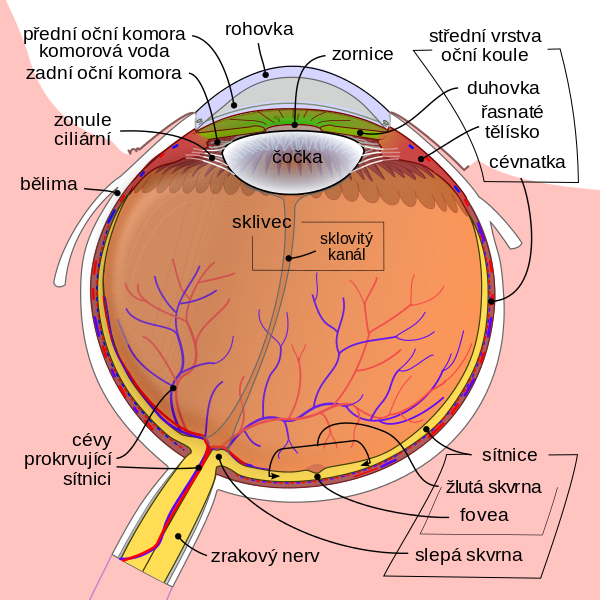
\includegraphics[width=.6\linewidth]{chap02_eye_anatomy}
    \caption{Schéma lidského oka \cite{pic_eye_anatomy}.}
    \label{pic:chap02_eye_anatomy}
  \end{center}
\end{figure}
\newpage 

\section{Sítnice}
\label{sec:sitnice}
Sítnice je nejdůležitější a také nejcitlivější částí našeho oka. Pokrývá ve formě tenké vrstvy zadní vnitřní stěnu oka. Obsahuje velké množství světločivných buněk, které umožňují vidění, a nervová vlákna. Sítnice zachycuje obraz a zrakovým nervem jej posílá do mozkové kůry. Onemocnění sítnice je vždy velmi závažné, často nevratné a může vést až ke ztrátě zraku.

\begin{itemize}
  \item\textbf{Světločivné buňky} tvoří základ fotoreceptorů. Jedná se o~buňky vytvářející nervovou stimulaci na základě absorpce fotonu přicházejícího na sítnici. Tyto buňky jsou dvojího typu: tyčinky a čípky. \textbf{Čípky} jsou citlivé na světlo různé barvy, čili různé vlnové délky, různé intenzity a různé sytosti barev. Jsou prvními neurony sítnice. Zajišťují barevné vidění za denního světla, jsou zodpovědné za zrakovou ostrost. Nacházejí se v~nejhojnějším počtu v~centrální jamce (fovea centralis) a směrem k~periferii sítnice jejich hustota postupně klesá. \textbf{Tyčinky} jsou světločivné buňky reagující na nižší intenzitu osvětlení než čípky, ale nejsou schopny rozeznávat barvy. Zajišťují noční vidění, tedy vnímání pouze jasu \cite{anatomie_oka}.
  \item\textbf{Žlutá skvrna} je struktura na sítnici představující místo nejostřejšího vidění, na kterém se tvoří obraz, když čteme nebo upřeně pozorujeme nějaký předmět. Ve svém středu obsahuje \textbf{foveu}, což je malá jamka, kde jsou nejhustěji obsaženy čípky a naopak hustota tyčinek je zde relativně malá. Z~tyčinek a čípků vycházejí nervová vlákna, která se nakonec spojují ve zrakový nerv.
  \item\textbf{Optický disk} je přibližně oválný útvar na sítnici, ve kterém vchází zrakový nerv dovnitř oční koule, tudíž neobsahuje žádné světločivné buňky. V~tomto místě se obraz netvoří, proto se také někdy nazývá slepá skvrna.
\end{itemize}

Jednotlivé části lze vidět na obrázku \ref{pic:chap02_retina}.
  
\vspace{10mm}

\begin{figure}[h]
  \begin{center}
    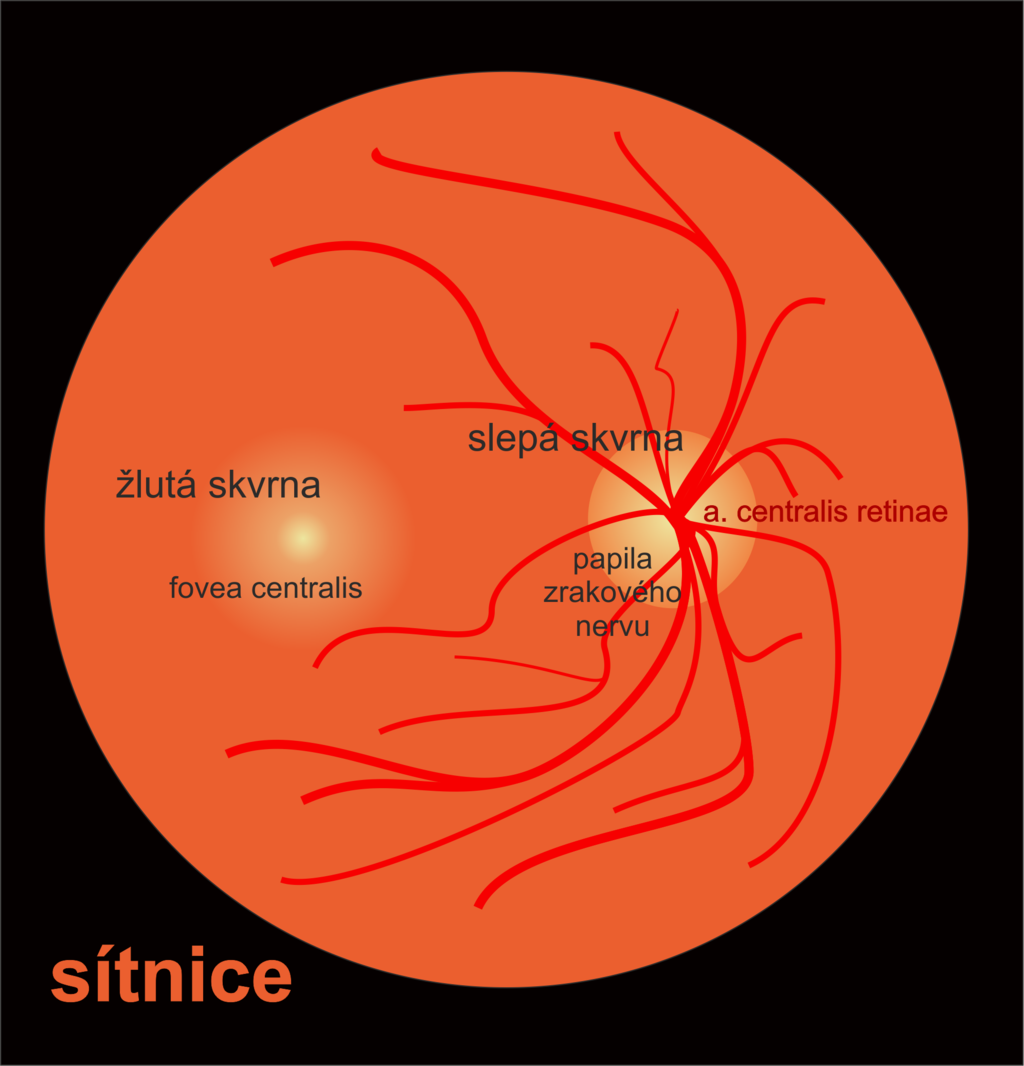
\includegraphics[width=.6\linewidth]{chap02_retina}
    \caption{Sítnice lidského oka \cite{pic_retina}.}
    \label{pic:chap02_retina}
  \end{center}
\end{figure}


\section{Vyšetření očního pozadí}
\label{sec:vysetreni}

\subsection*{Oftalmologie}
Oftalmologie je odvětví medicíny zabývající se anatomií, fyziologií, onemocněními oční bulvy a chirurgií zrakových drah, jež zahrnují oko, mozek a oblasti okolo mozku, jako je slzný systém nebo oční víčka. Jedná se o~velice úzce specializovaný obor, především vzhledem k~tomu, že oko je velmi komplikovaný aparát. Oční lékař je specialistou na lékařské a chirurgické onemocnění očí.


\subsection*{Štěrbinová lampa}
Štěrbinová lampa je nejpoužívanější přístroj v~očním lékařství. Jedná se o~speciální mikroskop, který umožňuje dokonalé vyšetření zejména předního segmentu oka: rohovky, duhovky, čočky, přední oční komory apod. Mikroskop je propojen s~lampou, jenž představuje světelný zdroj procházející úzkou štěrbinou. Lékař světlo zamíří pacientovi přímo do oka, a tak přesně nasvítí vyšetřovanou oblast. Při vyšetření jsou tkáně osvětleny buď přímým proužkem světla nebo je tkáň osvětlena zpětně odraženým světlem. Prohlížením nasvíceného oka pomocí mikroskopu pak lékař získá mnohonásobně zvětšený obraz pozorované oblasti, díky čemuž může zachytit i velmi jemné změny a příznaky očních onemocnění.

\subsection*{Oftalmoskopie}
Oftalmoskopie je vyšetření očního pozadí oftalmoskopem. Jedná se o~lékařskou pomůcku, která používá světelného paprsku, jenž je nasměrován do oka malým zrcadlem nebo hranolem a umožňuje jeho prohlédnutí. Oftalmoskopem je možné sledovat změny na cévách očního pozadí, cévnatce, sítnici i na zrakovém nervu. Rozšíření zorniček neboli mydriáza je jednoduchý a efektivní způsob, jak lze lépe pozorovat struktury za nimi. To se často provádí pomocí očních kapek před samotným vyšetřením. Existují dva hlavní typy oftalmoskopie. 

\begin{itemize}
  \item\textbf{Přímá oftalmoskopie} využívá přímého oftalmoskopu, který vytváří vzpřímený obraz přibližně 15násobného zvětšení. Jedná se o~malý přenosný nástroj, který můžete vidět na obrázku \ref{pic:chap02_ophthalmoscope_direct}. Světelný zdroj je umístěn v~horní části přístroje pod otvorem určeným pro pozorování. Sítnice se sleduje z~krátké vzdálenosti jedním okem. Tento typ oftalmoskopu se nejčastěji používá při rutinním vyšetření očního pozadí. Vyšetření se nejlépe provádí v~tmavé místnosti. Přímou oftalmoskopií lze pozorovat například degeneraci makuly. 
  \item\textbf{Nepřímé oftalmoskopie} umožňuje pozorovat větší oblasti očního pozadí v~obráceném obrazu s~2 až 5násobným zvětšením. Poskytuje širší pohled na vnitřní oko. Nepřímý oftalmoskop (obrázek \ref{pic:chap02_ophthalmoscope_indirect}) užívá speciálně upravený zdroj světla, který je umístěný na čelence, a přidaných čoček lupy, které jsou kladeny do blízkosti oka. To umožňuje vyšetření sítnice z~větší vzdálenosti. Nepřímý oftalmoskop poskytuje silnější světelný zdroj, speciálně konstruovaný objektiv a možnost stereoskopické kontroly vnitřku oční bulvy. Zornice musí být plně rozšířeny pro uspokojivý výsledek. Používá se k~perifernímu sledování sítnice pro pozorování nitroočních zánětů, u~cévních mozkových příhod, roztroušené sklerózy, nitrolební hypertenze aj.
\end{itemize}

\begin{figure}[h]
  \begin{minipage}[c]{0.47\textwidth}
    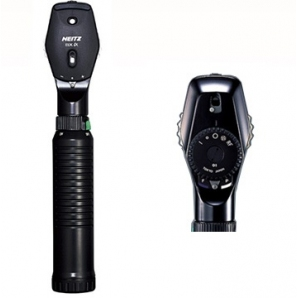
\includegraphics[width=\linewidth]{chap02_ophthalmoscope_direct}
    \caption{Přímý oftalmoskop \cite{pic_dir_scope}.}
    \label{pic:chap02_ophthalmoscope_direct}
  \end{minipage}
  \hfill
  \begin{minipage}[c]{0.47\textwidth}
    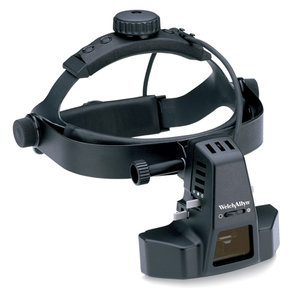
\includegraphics[width=\linewidth]{chap02_ophthalmoscope_indirect}
    \caption{Nepřímý oftalmoskop \cite{pic_indir_scope}.}
    \label{pic:chap02_ophthalmoscope_indirect}
  \end{minipage}
\end{figure}
  

\subsection*{Fundus kamera}
Fundus kamera (obrázek \ref{pic:chap02_fundus_camera}) je přístroj nahrazující oftalmoskop. Je založena na principu monokulární nepřímé oftalmoskopie. Fundus kamera poskytuje vzpřímený, zvětšený záběr na oční pozadí. Typická kamera zobrazuje 30 až 50$^\circ$ oblasti sítnice se zvětšením 2,5$\times$ a umožňuje změnu tohoto vztahu pomocí zoomu nebo pomocných čoček. Optika fundus kamery je podobná optice nepřímého oftalmoskopu v~tom, že pozorovací a osvětlovací systémy následují odlišné cesty. Jejím výstupem jsou digitální obrazy sítnice, které se používají pro sledování stavu sítnice a případnou diagnostiku očních onemocnění. Použití této kamery je neinvazivní, tedy nijak nezasahuje do snímaného oka. Před vyšetřením se aplikují oční kapky na rozšíření zornic \cite{pristroje}.

\begin{figure}[h]
  \begin{center}
    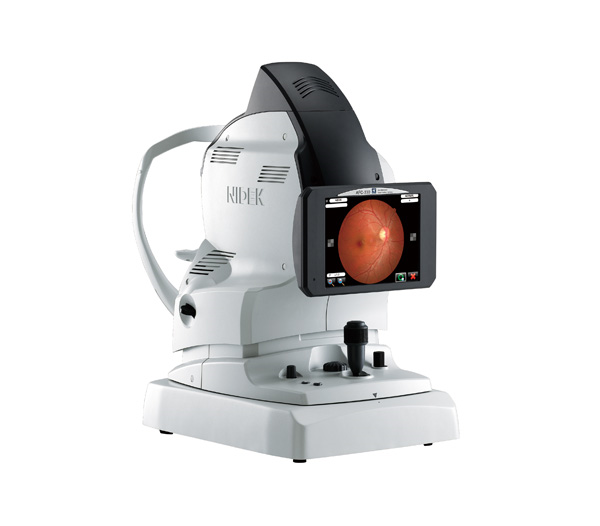
\includegraphics[width=0.7\linewidth]{chap02_fundus_camera}
    \caption{Fundus kamera \cite{pic_fundus}.}
    \label{pic:chap02_fundus_camera}
  \end{center}
\end{figure}
  \chapter{Onemocnění sítnice lidského oka}
\label{ch:nemoci}

\section{Věkem podmíněná makulární degenerace}
Věkem podmíněná makulární degenerace (dále jen VPMD) je onemocnění makuly, které se objevuje u~pacientů starších 50 let a je nejčastější příčinou praktické slepoty v~ekonomicky vyspělých zemích. S~rostoucím počtem seniorů se stává velkým celospolečenským zdravotním problémem. Na vznik a rozvoj tohoto onemocnění má vliv více faktorů. Kromě rostoucího věku to může být i vysoký krevní tlak, kouření, špatné stravovací návyky a s~tím spojená obezita a genetické dispozice. Pacienti popisují její projevy tak, že zraková ostrost postupně klesá, stěžují si na deformace obrazu a v~pokročilejších případech se v~centru zorného pole objevuje rozmazaná nebo někdy až černá skvrna. Rovněž dochází ke zhoršení barevného vidění. Léčitelná je jeho vlhká forma, kdy současná medicína dokáže pouze mírně zpomalit její projevy. Ke zlepšení zraku již nedojde a pouze se stabilizuje aktuální kvalita vidění \cite{Atlas}.

\subsection*{Formy věkem podmíněné makulární degenerace}
VPMD rozdělujeme na 2 formy: suchou (atrofickou, nonexsudativní) a vlhkou (exsudativní). Suchou formou je postiženo až 90 \% pacientů, ale jen u~12--21 \% způsobuje závažnou poruchu zraku. Vlhkou formou trpí méně pacientů, ale je daleko závažnější než suchá forma, protože postupuje velmi rychle. Obě dvě formy se mohou v~průběhu onemocnění kombinovat. V~makulární krajině nemocných nacházíme změny a úbytek retinálního pigmentového epitelu a drúzy. Drúzy dělíme podle vzhledu a velikosti na tvrdé a měkké. Jejich porovnání lze vidět na obrázcích \ref{pic:chap03_drusen_hard} a \ref{pic:chap03_drusen_soft}. Tvrdé drúzy jsou malá ohraničená depozita žlutavé barvy. Naopak měkké drúzy nemají ostré ohraničení a mohou i splývat, jsou spojeny s~podstatně vyšším rizikem vzniku vlhké formy VPMD. Další možnou úlohu při tvorbě drúz hrají lipidy, které se ukládají v~Bruchově membráně a brání výměně živin \cite{vpmd_kolar}.

\begin{figure}[h]
  \begin{minipage}[c]{0.47\textwidth}
    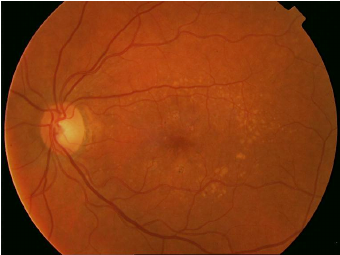
\includegraphics[width=\linewidth]{chap03_drusen_hard}
    \caption{Tvrdé drúzy \cite{vpmd_kolar}.}
    \label{pic:chap03_drusen_hard}
  \end{minipage}
  \hfill
  \begin{minipage}[c]{0.47\textwidth}
    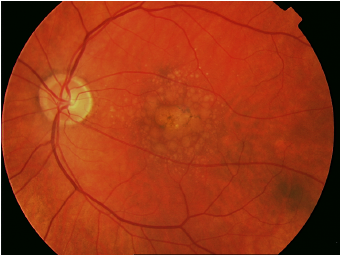
\includegraphics[width=\linewidth]{chap03_drusen_soft}
    \caption{Měkké drúzy \cite{vpmd_kolar}.}
    \label{pic:chap03_drusen_soft}
  \end{minipage}
\end{figure}


\begin{itemize}
  \item\textbf{Suchá forma} se často projevuje velmi pomalým postupným zhoršováním ostrosti vidění v~průběhu let. Včasná fáze začíná poškozením pigmentové vrstvy sítnice, která zabezpečuje metabolizmus sítnice, následně hromadění odpadních látek ve formě drúz a projevem určitého stupně atrofie. Mezi první příznaky patří rozmazané vidění, zhoršené vidění za tmy či za soumraku, zhoršení možnosti čtení nebo zaostření na jeden objekt. Geografická atrofie představuje rozvinuté stadium suché formy VPMD. Vidět ji můžete na obrázku \ref{pic:chap03_geo_atrof}. K~příznakům raného stádia patří měkké drúzy, hypopigmentace spojená s~drúzami a hyperpigmentace spojená s~drúzami. Léčba suché formy VPMD v~současné době není k~dispozici. Avšak na zastavení nebo zpomalení její progrese může mít příznivý vliv doplnění antioxidačních vitamínů C, E a minerálů zinek, selen a esenciálními omega-3 nenasycenými mastnými kyselinami. Podpůrnou úlohu má i strava bohatá na ryby, listovou zeleninu a ovoce \cite{vpmd_kolar}.
  
  \begin{figure}[h]
    \begin{center}
      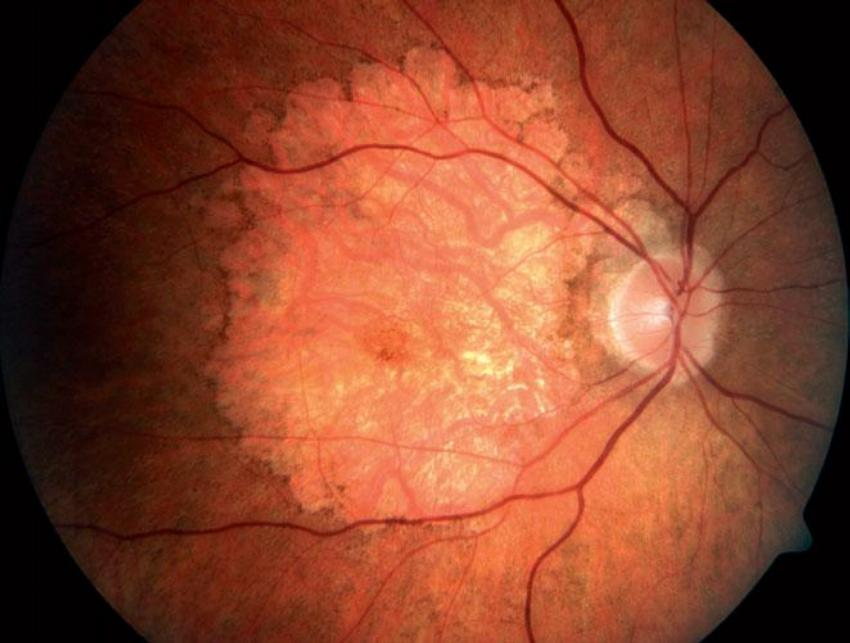
\includegraphics[width=.6\linewidth]{chap03_geo_atrof}
      \caption{Geografická atrofie \cite{pic_geo_atrof}.}
      \label{pic:chap03_geo_atrof}
    \end{center}
  \end{figure}

  \item\textbf{Vlhká forma} v~porovnání se suchou formou postupuje rychleji a ztráta vidění je výraznější. K~rapidnímu zhoršení dochází v~průběhu několika týdnů a k~praktické slepotě již během pár měsíců. Je způsobena podrůstáním nových cév pod sítnici, které postupně začínají prosakovat, a tím způsobí otok nebo krvácení. Prosakování a krvácení stimuluje tvorbu vazivové tkáně a v~makule se vytvoří útvar, který se nazývá pseudotumor. Základními projevy onemocnění jsou deformace vnímaného obrazu, výpadek zejména centrální části zorného pole, pokles centrální zrakové ostrosti hůře vnímaný do blízka a charakteristický nález na očním pozadí (viz obrázek \ref{pic:chap03_soft_armd}). Onemocnění vede k~úplné ztrátě centrálního vidění, periferní vidění je zachováno. Léčba dříve spočívala v~destrukci neovaskulární membrány fotokoagulačním nebo termoterapeutickým laserem. Výsledky léčby však byly kolísavé. Východiskem měla být cílenější tzv. fotodynamická terapie, při které je nitrožilně podaná látka absorbována cílovou tkání a poté aktivována laserem \cite{vpmd_kolar}.
  
  \begin{figure}[h]
    \begin{center}
      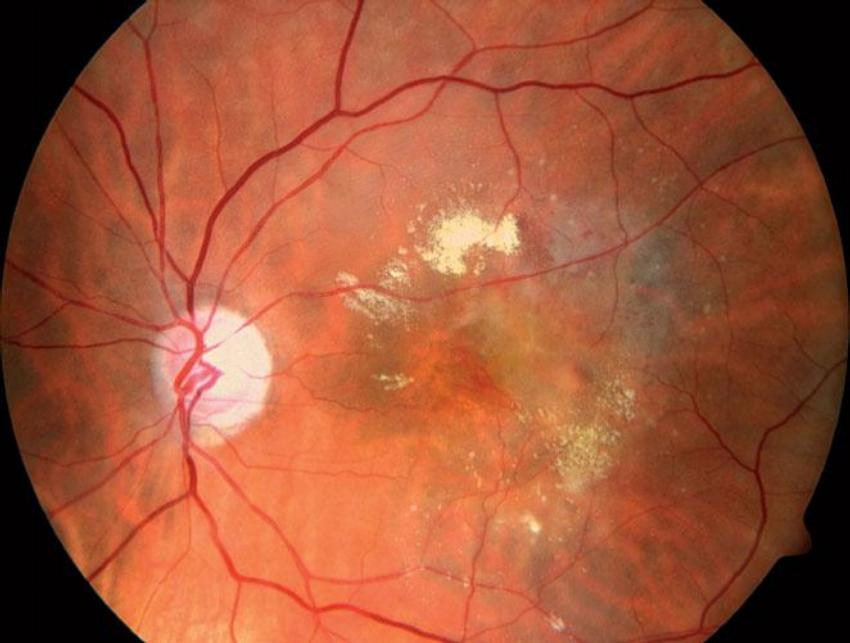
\includegraphics[width=0.6\linewidth]{chap03_soft_armd}
      \caption{Vlhká forma s~edémem \cite{pic_soft_armd}.}
      \label{pic:chap03_soft_armd}
    \end{center}
  \end{figure}

\end{itemize}


\section{Retinopatie}
V~souvislosti s~celkovými onemocněními, jako je vysoký krevní tlak nebo arterioskleróza, se mohou rozvíjet trvalé změny na sítnici, které nazýváme retinopatie. Dochází postupně ke zužování cév a poklesu krevního zásobení sítnice až k~postižení zrakového nervu a nevratným změnám.  

Zvláštním případem retinopatie je retinopatie diabetická. Projeví se asi po 8--10 letech trvání cukrovky. Pacient zaznamenává výpadky zorného pole nebo pokles zrakové ostrosti. Na tento typ onemocnění navazuje celá řada komplikací jako je zánět duhovky, šedý zákal, zánět nervů apod. Předpokladem úspěšné léčby diabetického poškození sítnice je především stabilizace cukrovky. Velmi často dochází k~degeneraci sítnice, což zahrnuje nezánětlivé změny na sítnici, které jsou spojeny s~poškozením nervových buněk. Vznikají na dědičném základě a postihují obvykle obě oči současně \cite{nemoci}.


\section{Odchlípení sítnice}
Jedná se o~velmi vážné onemocnění, které může postihnout člověka v~jakémkoliv věku, nejčastěji jsou tímto onemocněním postiženi jedinci středního a staršího věku. Projevuje se záblesky před očima, drobnými tečkami či tmavým stínem v~zorném poli. K~odchlípení sítnice oka dochází, když se v~sítnici objevují různé trhlinky, které způsobují, že tekutina ze sklivce se začne dostávat pod sítnici a nadzvedávat ji (tím se sítnice odlučuje od vrstvy pigmentových buněk). Díky tomu se pak do sítnice nedostávají živiny a kyslík, a proto buňky přítomné v~sítnici rychle odumírají. Nejčastěji k~tomuto odchlípnutí dochází na okraji sítnice, odtud se ale při neléčení pomalu přesouvá i do centra vidění. V~některých případech odchlípnutí sítnice způsobilo i svrašťování sklivce, k~němuž běžně dochází v~rámci stárnutí člověka. Při stárnutí (někdy i při úrazu, nebo krátkozrakosti či zánětu) vznikají v~sítnici drobná ložiska, která mohou vytvářet nové spojení mezi sklivcem a sítnicí. Právě tato spojení způsobují, že může dojít k~vytržení části sítnicové tkáně, když se sklivec smršťuje. 

Pokud lékař objeví trhliny nebo díry v~sítnici ještě před vznikem odchlípnutí, využívá se laserová koagulace, kterou se sítnice připojí k~ostatním vrstvám oční stěny. Pokud již ale k~odchlípnutí sítnice došlo, jediným řešením je operace pod celkovou anestezií \cite{nemoci}.  


\section{Prasklá sítnice}
Sítnice může v~oku člověka prasknout z~různých důvodů. Může to být důsledek komplikací jiného očního onemocnění, může se jednat o~degenerativní formu onemocnění očí nebo k~tomu může dojít také při poranění očí či mozku. K~tomuto prasknutí dochází obvykle v~důsledku toho, že sítnice není delší dobu správně prokrvována. Vliv na prasknutí může mít i stáří oční bulvy.
Pokud se jedná o~drobné prasklinky v~sítnici, tak si pacient nemusí uvědomovat žádné problémy se zrakem, ale i přesto na sobě může postupně vypozorovat různé příznaky jako světlé záblesky před očima, zužování viditelného pole a další. Pokud je ale sítnice oka porušená výrazněji může dojít k~výraznému zhoršování zraku, i k~jeho ztrátě.

Léčba praskliny může probíhat pomocí laseru, kryoterapií i chirurgickým zákrokem. O~formě léčbu rozhoduje vždy lékař v~závislosti na rozsahu, typu a umístění praskliny.


\section{Zánět sítnice}
Toto onemocnění je také známé pod označení retinitida. Projevuje se rozmazaným viděním a pohyblivými skvrnami v~zorném poli. Typická je také vysoká citlivost na světlo a slzení. Zánět sítnice oka mohou způsobit viry i paraziti, nejčastější příčinou jsou ale bakterie. Pacientovi se infekce do sítnice může dostat krví ze zánětlivého ložiska v~podstatě kdekoliv v~těle. Sítnice se může zanítit i po úrazu nebo v~případě, kdy je infekce do oka zanesena přímo (například promnutí oka rukou). Když tělo léčí tuto infekci, tak imunitní buňky poškozují současně i buňky v~sítnici, což může vést ke zhoršování zraku. V~mnoha případech není zánět sítnice osamocený a doprovází ho také zánět cévnatky, která sítnici zásobí krví.

K~léčbě zánětu sítnice oka obvykle lékař předepíše antibiotika, v~závažnějších případech může předepsat i kortikoidy. Obvykle záleží na tom, co zánět způsobilo. Antibiotika se samozřejmě nepředepisují v~případě, že onemocnění způsobily viry, v~takovém případě se nasazují antivirotika.


\section{Otok sítnice}
Otok sítnice neboli diabetický makulární edém postihuje, jak již název napovídá, diabetiky. K~tomuto otoku dochází po prosáknutí makuly tekutinou. Otok sítnice způsobuje, že se snižuje schopnost vnímat světlo. Díky tomu  má pacient rozmazané vidění a není schopen zaostřit oko. Tento otok se může objevit u~lidí, kteří cukrovkou trpí dlouhodobě, nebo pokud i při léčbě mají příliš vysokou hladinu glukózy. Otok je způsoben poškozením cév v~sítnici a jejím okolí. Tyto cévky pak propouštějí tekutinu do sítnice, kde se hromadí, a tím vzniká otok.

Pokud by nedošlo k~léčbě, může otok sítnice vést až k~úplné ztrátě zraku. Léčba otoku sítnice musí probíhat v~závislosti na léčbě cukrovky,  kdy se hladina cukru v~krvi udržuje ve vhodných hodnotách. Otok sítnice se obvykle léčí laserovou operací očí, kdy se laserem spálí prosakující cévy, a tím se uzavřou.


\section{Oběhové poruchy sítnice}
Poměrně častým onemocněním sítnice jsou oběhové poruchy, kdy dochází k~uzávěru sítnicových cév. Tyto uzávěry vznikají většinou jako důsledek arteriosklerózy, což je degenerativní onemocnění cév, kde dochází k~jejím zužování a k~horšímu krevnímu zásobení tkání. Vznik arteriosklerózy je podporován některými celkovými chorobami jako je vysoký krevní tlak, cukrovka, porucha metabolismu tuků apod \cite{nemoci}.

Při \textbf{uzávěru centrální sítnicové tepny} dochází k~náhlému zhoršení vidění. Na očním pozadí je vidět zúžená tepna, dochází k~nedokrvení a otoku sítnice. Je důležité, aby byla léčba zahájena včas, nejlépe do dvou hodin od vzniku prvních příznaků. Aplikují se léky na rozšíření cév, léky na rozpuštění trombu a léky zabraňující srážení krve. I~přes včasnou léčbu bývá funkce sítnice často snížena.

\textbf{Uzávěr centrální sítnicové žíly} se projevuje rychlým zhoršováním vidění, trombus způsobuje přetlak žíly, rozšíření žíly je nepravidelné a dochází ke krvácení do sítnice. Podávají se léky na rozšíření cév, po čase se tromby vstřebávají, popřípadě se pomocí laseru zlepšují oběhové poměry v~sítnici.

  \chapter{Zpracování obrazu}
\label{ch:techniky}
Pro úspěšné vytvoření algoritmu na detekci chorob na sítnici lidského oka je nutné znát jednak konkrétní projevy daných onemocnění, které jsou popsány v~předchozí kapitole, ale také nejrůznější metody zpracování digitálního obrazu. V~této kapitole jsou popsány základní algoritmy z~této oblasti a z~oblasti počítačového vidění.

Máme k~dispozici digitální obraz sítnice. Ten však může být různými způsoby zkreslen (například díky způsobu snímání nebo nevhodným podmínkám při jeho průběhu) a tím pádem nepříznivě ovlivnit detekci. Pro co nejpřesnější a nejlepší výsledky musíme před samotným zahájením procesu detekce provést úpravu tohoto digitálního obrazu. Základní změny, které můžeme provést pro prvotní zpracování obrazu jsou vyhlazování obrazu, prahování a morfologické operace.

\section{Vyhlazování obrazu}
\label{sec:smoothing}
Vyhlazování obrazu používáme pro odstranění nežádoucích artefaktů v~obraze jako je například šum, který může navozovat dojem, jako kdyby obraz zrnil. Existuje mnoho metod pro vyhlazování obrazu, kde každá metoda řeší jiný druh šumu. Tyto metody se také liší svou výpočetní náročností a efektivitou v~odstraňování konkrétního druhu šumu.
\begin{itemize}
  \item \textbf{Průměrování} je konvoluce obrazu s~normalizovanou maskou. Každý pixel překrytý touto maskou vynásobíme koeficientem v~příslušné buňce a provedeme součet všech těchto hodnot. Tím se získá jeden nový pixel. Výšku a šířku této masky lze specifikovat. Konvoluční maska 3$\times$3 by vypadala následovně:
  
  $$
    \text{K} = \frac{1}{9}\left\lbrack
    \begin{array}{ccc}
      1 & 1 & 1\\
      1 & 1 & 1\\
      1 & 1 & 1\\
    \end{array} \right\rbrack
  $$

  \item \textbf{Gaussovo vyhlazování} je jednou z~metod odstranění šumu využívající konvoluce obrazu s~maskou, která se skládá z~elementů určených Gaussovou funkcí. Ty slouží pro výpočet transformací, které se aplikují na každý pixel v~obraze. Gaussovo vyhlazování je velmi efektivní technika v~odstraňování Gaussovského šumu, který odpovídá Gaussovu rozložení. Tento šum si lze prohlédnout na obrázku \ref{pic:chap04_lenna_gauss_noise}. Rovnice Gaussovy funkce ve dvou dimenzích \cite{comp_vision}:

  \begin{equation}
    G(x,y)=\frac{1}{2\pi\sigma^2}e^{-{\frac{x^2+y^2}{2\sigma^2}}}
  \end{equation}

  kde $x$ a $y$ jsou souřadnice v~obraze a $\sigma$ je směrodatná odchylka Gaussovy distribuce. Ukázka Gaussovy matice je zobrazena na obrázku \ref{pic:chap04_gaussian_matrix}.
  
  \begin{figure}[h]
	\begin{center}
		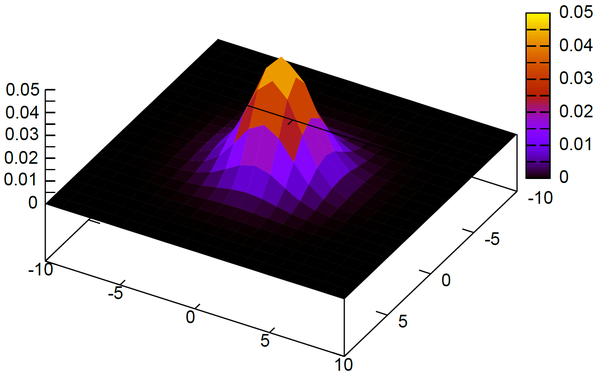
\includegraphics[width=0.75\linewidth]{chap04_gaussian_matrix}
		\caption{Gaussova matice (okolí 10 pixelů, odchylka 1,8) \cite{pic_gauss_matrix}.}
		\label{pic:chap04_gaussian_matrix}
	\end{center}
  \end{figure}

  \item \textbf{Mediánové vyhlazování} vymezí pro každý pixel obrazu jeho okolí. Ze všech těchto pixelů vybere medián, který se stává novou hodnotou zpracovávaného pixelu. To je vysoce účinné pro odstraňování šumu typu sůl a pepř, který je viditelný na obrázku \ref{pic:chap04_lenna_salt_pepper}. Ve výše uvedených filtrech je centrálním prvkem nově vypočtená hodnota, která může být existující hodnotou pixelu v~obraze nebo zcela novou hodnotou. Při mediánovém vyhlazování je centrální prvek vždy nahrazen hodnotou nějakého pixelu v~obraze.
  
  \begin{figure}[h]
    \begin{minipage}[c]{0.47\textwidth}
      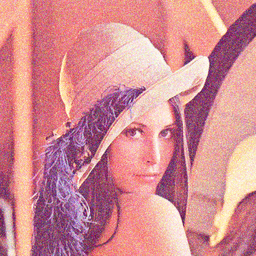
\includegraphics[width=\linewidth]{chap04_lenna_gauss_noise}
      \caption{Gaussovský šum \cite{pic_lenna}.}
      \label{pic:chap04_lenna_gauss_noise}
    \end{minipage}
    \hfill
    \begin{minipage}[c]{0.47\textwidth}
      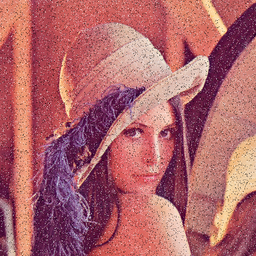
\includegraphics[width=\linewidth]{chap04_lenna_salt_pepper}
      \caption{Šum typu sůl a pepř.}
      \label{pic:chap04_lenna_salt_pepper}
    \end{minipage}
  \end{figure}

\end{itemize}

\section{Prahování}
Prahování neboli tresholding je nejjednodušší metoda segmentace digitálního obrazu založená na hodnocení intenzity jednotlivých pixelů. Jejím principem je nalezení takové hodnoty prahu (threshold), pro kterou bude platit, že všechny hodnoty intenzity vyšší než práh odpovídají popředí, zatímco všechny hodnoty nižší než práh odpovídají pozadí. V~případě, že se rozložení intenzity pixelů popředí a pozadí výrazně překrývá, může být nalezení vhodné hodnoty prahu prakticky nemožné. Z~obrázku ve stupních šedi lze prahováním vytvořit binární (černobílý) obraz. Je to metoda jednoduchá a rychlá, ale relativně destruktivní pro výsledný obraz. Binární prahování lze vyjádřit následujícím vztahem \cite{izg}:
\begin{equation}
  P(x,y) = \left\{
  \begin{array}{l l}
    1 & \text{pro} \quad I(x,y) \geq T\\
    0 & \text{pro} \quad I(x,y) < T
  \end{array} \right.
\end{equation}

\textbf{Adaptivní prahování} je možné využít v~případech, kdy má zpracovávaný obraz odlišné světelné podmínky v~různých oblastech, což znemožňuje přímo určit jeden globální práh. Tato metoda rozdělí obraz na menší části, pro každou vypočte prahovou hodnotu a následně provede binární prahování jednotlivých oblastí. Tímto způsobem se docílí lepších výsledků u~obrazů s~různým osvětlením. Rozdíl mezi binárním a adaptivním prahováním lze pozorovat na obrázcích \ref{pic:chap04_lenna_thresh_bin} a \ref{pic:chap04_lenna_thresh_ada}.

\begin{figure}[h]
  \begin{minipage}[c]{0.47\textwidth}
    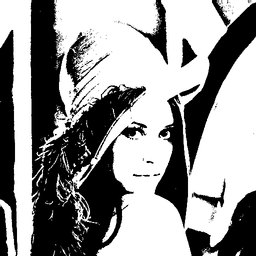
\includegraphics[width=\linewidth]{chap04_lenna_thresh_binary}
    \caption{Binární prahování s~globálním prahem.}
    \label{pic:chap04_lenna_thresh_bin}
  \end{minipage}
  \hfill
  \begin{minipage}[c]{0.47\textwidth}
    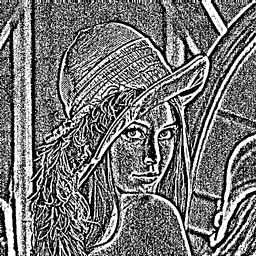
\includegraphics[width=\linewidth]{chap04_lenna_thresh_adaptive}
    \caption{Adaptivní Gaussovo prahování.}
    \label{pic:chap04_lenna_thresh_ada}
  \end{minipage}
\end{figure}

\textbf{Distribuce chyby} je další metoda převodu obrazu ve stupních šedi na černou a bílou, která je v~základu založena na metodě prahování. K~tomu je přidána distribuce vznikajících chyb okolním, dosud nezpracovaným pixelům. Je-li aktuální pixel převeden na černý, pak se vzniklá chyba rovná původní hodnotě pixelu. Je-li aktuální pixel převeden na bílou, pak se vzniklá chyba rovná rozdílu maximální hodnoty obrazu a původní hodnoty pixelu \cite{izg}.

\pagebreak
\section{Morfologické operace}
Matematická morfologie vychází z~vlastností bodových množin. Nejčastěji se aplikuje na binární obrazy, ale lze ji snadno zobecnit i na šedotónové a barevné obrazy. Morfologické operace se používají pro předzpracování (odstranění šumu, zjednodušení tvaru objektů), zdůraznění struktury objektů (kostra, ztenčování, zesilování, konvexní obal, označování objektů) a pro popis objektů číselnými charakteristikami (plocha, obvod, projekce, atd.).

Morfologické operace jsou realizovány jako relace obrazu (bodové množiny X) s~jinou menší bodovou množinou B, tzv. strukturním elementem. Morfologickou transformaci si lze představit jako určitý systematický pohyb strukturního elementu B po obrazu X a vyhodnocení odezvy podle typu operace. Mezi dvě základní morfologické operace patří dilatace a eroze.

\textbf{Dilatace} skládá body dvou množin pomocí vektorového součtu. Objekty v~obraze jsou po aplikaci dilatace zvětšené na úkor pozadí. Dilatace se používá k~zaplnění děr popř. zálivů a její definiční vztah je dán následujícím vzorcem \cite{feec}:

\begin{equation}
X \oplus B = \{d \in E^2 : d = x + b, x \in X, b \in B\}
\end{equation}

\textbf{Eroze} skládá dvě bodové množiny s~využitím vektorového rozdílu. Je duální (nikoliv inverzní) transformací k~dilataci a používá se pro zjednodušení struktury objektů. Objekty jednotkové tloušťky (relativní jednotka) zmizí a složité objekty spojené čárami jednotkové tloušťky se rozloží na několik jednodušších objektů. Eroze je dána následujícím vzorcem \cite{feec}:

\begin{equation}
X \Theta B = \{d \in E^2 : d + b \in X \text{ pro } \forall b \in B\}
\end{equation}

  \begin{figure}[h]
	\begin{center}
		
\includegraphics[width=.75\linewidth]{chap04_morph_overview}
		\caption{Základních morfologické operace.}
		\label{pic:chap04_morph_overview}
	\end{center}
  \end{figure}

Další morfologické operace jsou \textbf{otevření} a \textbf{uzavření} a jsou to operace, které vzniknou vzájemnou kombinací elementárních operací dilatace a eroze. Výsledkem obou je zjednodušený obraz, který obsahuje méně detailů (odstraní detaily menší než strukturní element, celkový tvar objektu se ale neporuší). Eroze následovaná dilatací se nazývá morfologické otevření, které je viditelné na obrázku \ref{pic:chap04_morph_open}. To oddělí objekty spojené úzkou šíjí, a tak zjednoduší strukturu objektů. Na obrázku \ref{pic:chap04_morph_close} je zobrazena dilatace následovaná erozí, která se naopak nazývá morfologické uzavření. Ta spojí objekty, které jsou blízko u~sebe, zaplní díry a vyhladí obrys \cite{feec}.

  \begin{figure}[h]
  \begin{minipage}[c]{0.47\textwidth}
    
\includegraphics[width=\linewidth]{chap04_morph_open}
		\caption{Morfologické otevření.}
		\label{pic:chap04_morph_open}
  \end{minipage}
  \hfill
  \begin{minipage}[c]{0.47\textwidth}
    
\includegraphics[width=\linewidth]{chap04_morph_close}
		\caption{Morfologické uzavření.}
		\label{pic:chap04_morph_close}
  \end{minipage}
\end{figure}

\pagebreak
\section{Momenty}
V~oblasti zpracování obrazu, počítačového vidění a souvisejících oborů je obrazový moment určitým váženým průměrem intenzity obrazových pixelů nebo funkcí takových momentů, obvykle vybraných tak, aby měly nějakou atraktivní vlastnost nebo interpretaci. Obrazové momenty jsou užitečné při popisu objektů po segmentaci. Jednoduché vlastnosti obrazu, které jsou pomocí nich získány, zahrnují oblast (nebo celkovou intenzitu), její těžiště a informace o~její orientaci. V~případě obrazu v~odstínech šedi a s~intenzitou pixelů $I(x,y)$ se momenty obrazu $M_{ij}$ vypočítají pomocí vztahu \cite{img_moments}:

\begin{equation}
M_{ij} = \sum_{x}\sum_{y} x^i y^j I(x,y)
\end{equation}

\noindent a následně můžeme vypočítat těžiště dané oblasti:

\begin{equation}
x = \frac{M_{10}}{M_{00}} \quad \text{a} \quad y = \frac{M_{01}}{M_{00}}
\end{equation}

\section{Houghova transformace}
Jedná se o~techniku extrakce vlastností. Jejím účelem je nalézt nedokonalé instance objektů v~rámci určité třídy tvarů pomocí hlasování. To se provádí v~prostoru parametrů, ze kterého jsou kandidáti objektů získání jako lokální maxima v~tzv. akumulačním prostoru, který je explicitně zkonstruován algoritmem při výpočtu Houghovy transformace. Klasická Houghova transformace byla určena pro identifikaci přímek v~obraze, ale později byla rozšířena pro určení pozic libovolných tvarů, nejčastěji kruhů nebo elips \cite{comp_vision}.

\section{Semínkové vyplňování}
Semínkové nebo také záplavové vyplňování slouží pro vyplnění dané oblasti ohraničené nějakým uzavřeným polygonem. Ze znalosti vnitřního bodu se určí, zda sousední body leží uvnitř oblasti nebo na její hranici. Podle způsobu určování sousedních bodů máme dva způsoby vyplňování, a to metodu používající čtyř sousedních bodů a metodu používající osmi sousedních bodů.

\subsection*{Algoritmus semínkového vyplňování}
Tento algoritmus má tři parametry: počáteční bod, hledanou barvu a cílovou barvu. Algoritmus vyhledá všechny body v~oblasti, které jsou připojeny k~počátečnímu bodu cestou hledané barvy, a změní je na cílovou barvu.
  \begin{enumerate}
    \item Pokud je barva bodu rovna cílové barvě, skonči.
    \item Pokud je barva bodu jiná než hledaná barva, skonči.
    \item Nastav barvu bodu na cílovou barvu.
    \item Znovu použij tento algoritmus pro všechny sousední body.
  \end{enumerate}

  \chapter{Návrh a implementace algoritmu}
\label{ch:navrh}
V~této kapitole bude představen navržený způsob detekce příznaků onemocnění na sítnici lidského oka a jeho implementace. Protože sítnice obsahuje různé struktury (žlutá skvrna, slepá skvrna a cévy), které nepředstavují nálezy a mohly by nepříznivě ovlivnit výsledek, je potřeba je také detekovat a z~celého procesu detekce příznaků onemocnění je vynechat. Tímto způsobem se zvýší přesnost tohoto algoritmu. Pořadí jednotlivých podkapitol odpovídá postupu výpočtu algoritmu.

\section{Předzpracování}
Pokud se podaří úspěšně načíst konkrétní snímek, je před dalším zpracováním změněna jeho vzorkovací frekvence. Hlavním důvodem je urychlení výpočtu, kde pokud se sníží celkový počet pixelů, které se mají zpracovat, sníží se tím i množství výpočtů, které je potřeba vykonat. Další výhodou je nastavování parametrů pro jednotlivé výpočty. Pokud jsou všechny vstupní snímky převedeny do určitého intervalu rozlišení, není potřeba definovat tyto parametry pro příliš široké spektrum rozlišení. V~tomto případě byl zvolen interval šířky obrázků od 2500~pixelů do 900~pixelů. Pokud má nějaký vstupní snímek na šířku větší počet pixelů než 2500, je provedeno snížení jeho vzorkování. Pro vytvoření jednoho nového pixelu je zapotřebí čtyř pixelů původních. Tímto způsobem se rozlišení obrázku sníží na polovinu --- bude mít poloviční šířku i poloviční výšku. Naopak pokud je nějaký vstupní obrázek užší než 900~pixelů, je provedeno zvýšení jeho rozlišení na dvojnásobek. Pokud některý ze snímků spadá do tohoto intervalu, je ponechán beze změny.

Dalším krokem je určení výše zmíněných parametrů výpočtů. Patří mezi ně velikost matice pro filtrování při získávání masky pozadí (filtr 1) a velikost matice pro filtrování při dalším zpracování (filtr 2). Tyto parametry jsou určeny na základě tří kategorií, které jsou dány intervalem šířky vstupních snímků. Přehled těchto hodnot lze vidět v~tabulce \ref{tab:parameters}. Díky úpravě rozlišení vstupních obrázku by měly všechny spadat do jedné z~těchto kategorií.

\begin{table}[ht]
  \begin{center}	
    \begin{tabular}{|c|c|c|}
      \hline
      \makecell{\textbf{Šířka snímku}\\\textbf{(v pixelech)}} & \makecell{\textbf{Filtr 1}\\\textbf{(v pixelech)}} & \makecell{\textbf{Filtr 2}\\\textbf{(v pixelech)}} \\
      \hline
      2500--1951 & 9$\times$9 & 13$\times$13 \\
      \hline
      1950--1401 & 7$\times$7 & 11$\times$11 \\
      \hline
      1400--900  & 5$\times$5 &  9$\times$9  \\
      \hline
    \end{tabular}
  \caption{Přehled parametrů výpočtů algoritmu.}
  \label{tab:parameters}
  \end{center}
\end{table}

\section{Získání masky pozadí}
Hlavním důvodem proč je potřeba oddělit pozadí snímku od popředí je efektivita. Při vyloučení pozadí z~následujícího zpracování dojde k~urychlení celkového výpočtu. Dalším důvodem je nežádoucí šum, který se na pozadí může objevit a který by mohl nepříznivě ovlivnit detekci.

Pro automatické oddělení masky pozadí od oblasti sítnice je potřeba nejprve převést výchozí snímek do odstínů šedé, aplikovat na něj vyhlazování pomocí průměrování normalizovanou maskou o~velikosti dané filtrem 1 (viz tabulka \ref{tab:parameters}) a následně zvolit takovou hodnotu prahu, která toto oddělení umožní. U~některých obrázků však pozadí není čistě černé a při zvolené hodnotě prahu, která fungovala pro většinu obrázků, se nedařilo oddělit pozadí snímku od sítnice. Z~toho důvodu je tato hodnota vypočítána pro každý snímek zvlášť.

Nejprve se získají čtvercové oblasti z~každého rohu obrázku, kde délka strany každé oblasti je rovna velikosti jedné desetiny výšky snímku. Následně se vypočítá průměrná intenzita jednotlivých oblastí a poté se vypočítá průměr těchto čtyř intenzit. Nakonec se tento průměr zaokrouhlí a přičte se k~němu hodnota 5. Tímto se získá velikost prahu.

Následným prahováním dojde k~již správnému oddělení pozadí od popředí. Pokud se ale v~pozadí objevovaly určité objekty jako například označení snímku, je potřeba tyto nežádoucí prvky odstranit. To je provedeno pomocí vyhledání kontur v~získané masce, kde největší kontura patří sítnici. Ta se ponechá a ostatní kontury se vyřadí. Při porovnání obrázků \ref{pic:chap05_background_mask_default} a \ref{pic:chap05_background_mask} je na první pohled jasné, která část obrazu patří pozadí a která sítnici.

\begin{figure}[h]
  \begin{minipage}[c]{0.47\textwidth}
    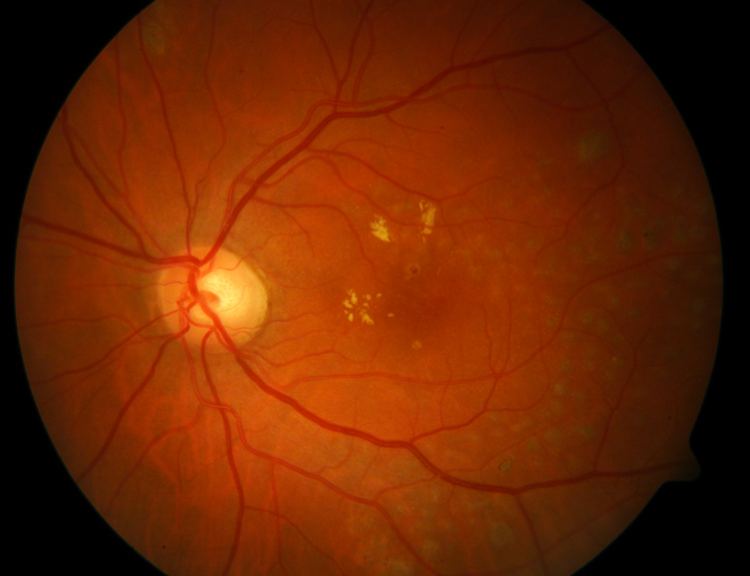
\includegraphics[width=\linewidth]{chap05_background_mask_default}
    \caption{Výchozí snímek.}
    \label{pic:chap05_background_mask_default}
  \end{minipage}
  \hfill
  \begin{minipage}[c]{0.47\textwidth}
    
\includegraphics[width=\linewidth]{chap05_background_mask}
    \caption{Maska pozadí.}
    \label{pic:chap05_background_mask}
  \end{minipage}
\end{figure}


\section{Získání vlastností oblasti sítnice}
Pro další výpočty u~algoritmů, které budou využity dále, je potřeba získat základní vlastnosti oblasti sítnice jako je střed a poloměr dané oblasti. K~jejich výpočtu je využita Houghova transformace pro hledání kružnic. Tento algoritmus pro extrakci vlastností je poměrně výpočetně náročný, ale vhodným nastavením mezních hodnot, kde se mají kružnice hledat, se celkový výpočet výrazně urychlí. Mezi tyto meze patří minimální vzdálenost mezi středy jednotlivých kružnic a dále minimální a maximální poloměr. Jako minimální vzdálenost mezi středy je zvolena větší hodnota z~počtu řádků a počtu sloupců snímku, kde se předpokládá, že požadovaná kružnice bude pouze jedna. Z~toho také vyplývá, že její průměr nemůže být větší než je počet těchto řádků nebo sloupců. Vydělením tohoto počtu dvěma získáme maximální poloměr. Minimální poloměr je vypočten ze vzorce pro obsah kružnice, kde je tento obsah dán velikostí oblasti sítnice. V~případě, že není dostupná maska pozadí a celý snímek je vyplněn sítnicí, pracuje se se středem snímku a jako poloměr je zvolena větší hodnota z~počtu řádků a počtu sloupců.


\section{Detekce optického disku}
Těžké exudáty vypadají podobně jako optický disk. Může se tedy stát, že při detekci dojde k~jejich záměně, a proto je potřeba ho detekovat a vyloučit z~dalšího zpracování. Optický disk je přibližně oválný útvar, který má na snímku sítnice často největší intenzitu. Díky této vlastnosti ho můžeme detekovat. Problém ale představují drúzy a exudáty, které mohou mít podobnou nebo dokonce větší intenzitu než optický disk. Z~tohoto důvodu se musí počítat i s~velikostí optického disku. Po experimentování nad databází snímků byl určen poloměr optického disku na hodnotu jedné sedminy poloměru oblasti sítnice. Hledá se tedy oblast s~určitou plochou nejjasnějších pixelů. 

Pro automatickou detekci optického disku je potřeba mít zpracovaný výchozí snímek. Z~něj se extrahuje zelený kanál, na kterém jde nejlépe vidět kontrast struktur na sítnici a jejího pozadí (viz obrázek \ref{pic:chap05_optic_disc_green_channel}). Z~něj se vypočítá oblast, ve které se bude hledat. Ta je tvořena pásem po celé šířce obrázku s~výškou odpovídající jedné pětině průměru oblasti sítnice. Tento pás lze vidět na obrázku \ref{pic:chap05_optic_disc_area}. Důvodem zmenšení oblasti, ve které se hledá optický disk, je eliminace nesprávných detekcí ve smímcích s~příliš velkým odleskem. Po získání této oblasti se provede vyhlazování pomocí průměrování normalizovaným filtrem 2 (viz tabulka \ref{tab:parameters}).

\begin{figure}[h]
  \begin{minipage}[c]{0.47\textwidth}
    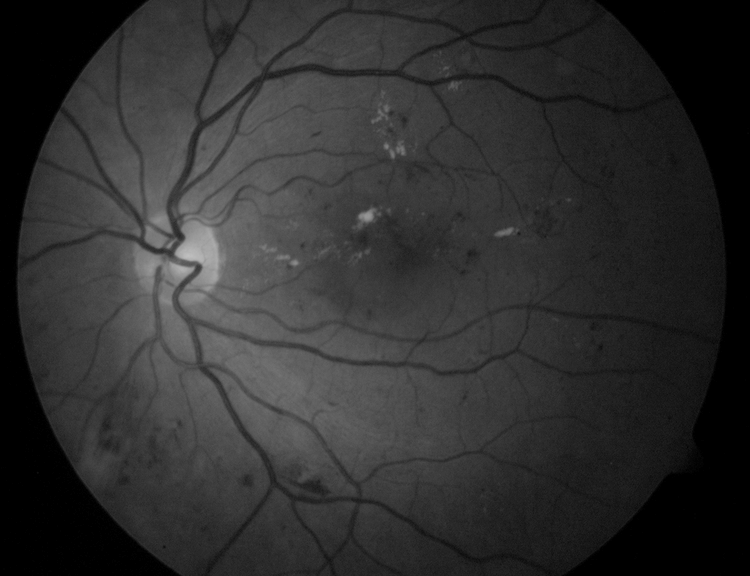
\includegraphics[width=\linewidth]{chap05_optic_disc_green_channel}
    \caption{Extrahovaný zelený kanál.}
    \label{pic:chap05_optic_disc_green_channel}
  \end{minipage}
  \hfill
  \begin{minipage}[c]{0.47\textwidth}
    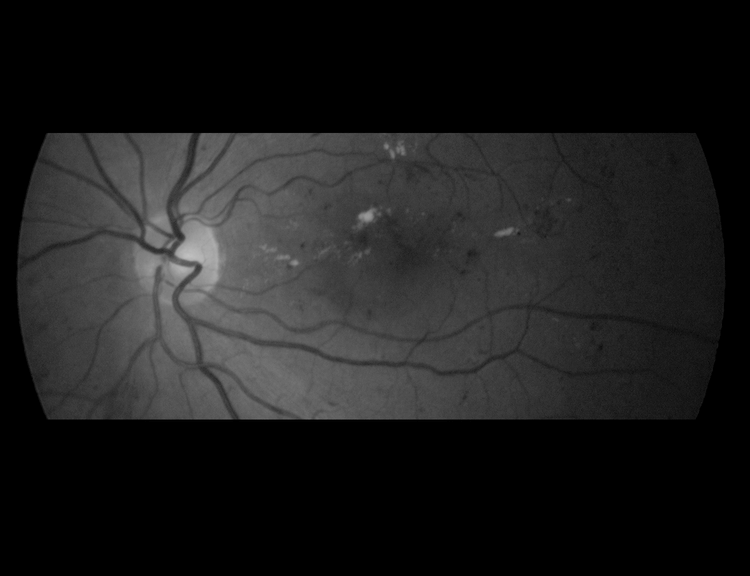
\includegraphics[width=\linewidth]{chap05_optic_disc_area}
    \caption{Zúžená oblast.}
    \label{pic:chap05_optic_disc_area}
  \end{minipage}
\end{figure}

Samotná detekce spočívá v~cyklickém binárním prahování, které začíná na maximální hodnotě 255 a postupně snižuje tento práh. Po každém prahování se ve snímku hledají kontury získaných oblastí, kterým se vypočítá jejich obsah. Kontuře, která obsahuje minimálně 11krát více pixelů než je poloměr oblasti sítnice, je vypočítána kružnice, která ji opisuje. Pokud je její poloměr menší nebo roven 1,2krát poloměru optického disku, pak mu tato oblast náleží. Těchto hodnot jsem dosáhl experimentováním nad databází snímků, kde vykazovaly největší úspěšnost. Výsledek posledního prahování je vidět na obrázku \ref{pic:chap05_optic_disc_thresh_area}.

Pomocí matematických momentů se vypočítá těžiště získané oblasti, které bude sloužit jako střed optického disku. Na základě umístění této oblasti se určí, zdali se jedná o~pravé či levé oko pacienta a podle toho se střed posune o~dvě pětiny svého poloměru daným směrem. Výsledek je na obrázku \ref{pic:chap05_optic_disc_result}.

\begin{figure}[h]
  \begin{minipage}[c]{0.47\textwidth}
    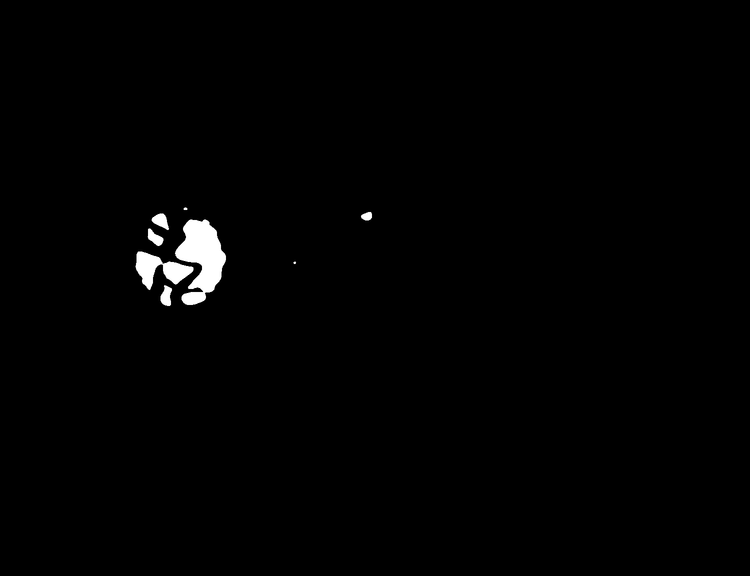
\includegraphics[width=\linewidth]{chap05_optic_disc_thresh_area}
    \caption{Konec binárního prahování.}
    \label{pic:chap05_optic_disc_thresh_area}
  \end{minipage}
    \hfill
  \begin{minipage}[c]{0.47\textwidth}
    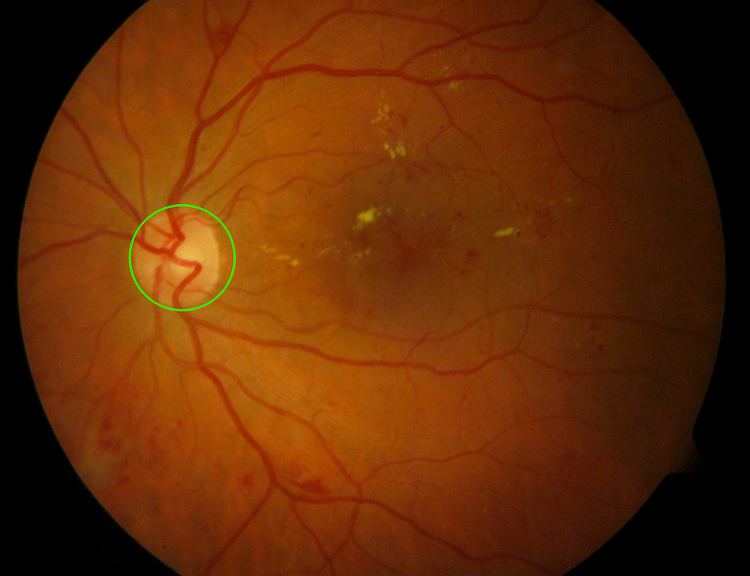
\includegraphics[width=\linewidth]{chap05_optic_disc_result}
    \caption{Detekovaný optický disk.}
    \label{pic:chap05_optic_disc_result}
  \end{minipage}
\end{figure}

Pro získání přesnější masky optického disku včetně menších oblastí, které mu náleží, se provádí dodatečné zpracování. Z~výchozího zeleného kanálu se extrahuje vypočítaná oblast optického disku (viz obrázek \ref{pic:chap05_optic_disc_mask_area}), která je průměrována normalizovanou maskou o~velikosti 5$\times$5~pixelů. Následně se provede jedno prahování s~hodnotou prahu o~2 nižší než je práh, při kterém došlo k~nalezení oblasti optického disku. Tímto způsobem se docílí daleko lepších výsledků. Rozdíl lze pozorovat na obrázcích \ref{pic:chap05_optic_disc_mask} a \ref{pic:chap05_optic_disc_mask_improved}.

\begin{figure}[h]
  \begin{minipage}[c]{0.315\textwidth}
    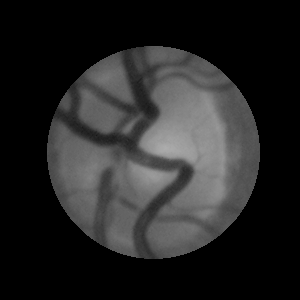
\includegraphics[width=\linewidth]{chap05_optic_disc_mask_area}
    \caption{Oblast optického disku.}
    \label{pic:chap05_optic_disc_mask_area}
  \end{minipage}
  \hfill
  \begin{minipage}[c]{0.315\textwidth}
    
\includegraphics[width=\linewidth]{chap05_optic_disc_mask}
    \caption{Nalezená oblast.}
    \label{pic:chap05_optic_disc_mask}
  \end{minipage}
    \hfill
  \begin{minipage}[c]{0.315\textwidth}
    
\includegraphics[width=\linewidth]{chap05_optic_disc_mask_improved}
    \caption{Výsledná maska.}
    \label{pic:chap05_optic_disc_mask_improved}
  \end{minipage}
\end{figure}


\section{Detekce fovey}
Abychom mohli správně klasifikovat příznaky VPMD, je potřeba detekovat foveu. Dalším důvodem, proč by se měla fovea detekovat, je možnost posouzení závažnosti onemocnění, neboť jak již bylo zmíněno dříve, fovea je struktura na sítnici představující místo nejostřejšího vidění. Díky tomu má největší vliv na kvalitu zraku a poškození právě této oblasti ji výrazně snižuje. Fovea je kruhovitá nebo oválná oblast, která je naopak oproti optickému disku jedním z~nejtmavších míst na sítnici. To v~některých případech může vést k~chybné detekci, kdy fovea splývá s~pozadím snímku nebo kdy je sítnice těžce poškozena. Na snímcích sítnice se fovea vždy vyskytuje relativně na stejném místě vzhledem k~optickému disku, a to přibližně ve dvou a půl násobku jeho šířky \cite{optic_disc}.

Při detekci fovey se opět pracuje se zeleným kanálem zdrojového snímku. Z~něho se vymezí zkoumaná oblast na základě posunutí středu optického disku pouze do vzdálenosti dvou a čtvrt násobku jeho průměru. Je to dáno tím, že poloměr optického disku je vypočítán tak, aby zahrnoval oblast o~něco větší, než je samotný disk. Poloměr zkoumané oblasti je pak 2krát větší než poloměr optického disku (viz obrázky \ref{pic:chap05_fovea_shift} a \ref{pic:chap05_fovea_area}). Zkoumaná oblast se následně vyhladí normalizovaným filtrem 2. Samotná detekce fovey je založená podobně jako u~detekce optického disku na cyklickém binárním prahování s~rozdílem, že hodnota prahu začíná na 0 a postupně se zvyšuje. Velikost hledané oblasti má i horní mez. Dolní mez je 6krát větší než poloměr oblasti sítnice a horní mez je 2,4krát větší než mez dolní. Tyto hodnoty byly získány také experimentováním nad databází snímků. První oblast, která spadá do těchto mezí, náleží fovey. Výsledek je zobrazen na obrázku \ref{pic:chap05_fovea_result}.

\begin{figure}[h]
  \begin{minipage}[c]{0.315\textwidth}
    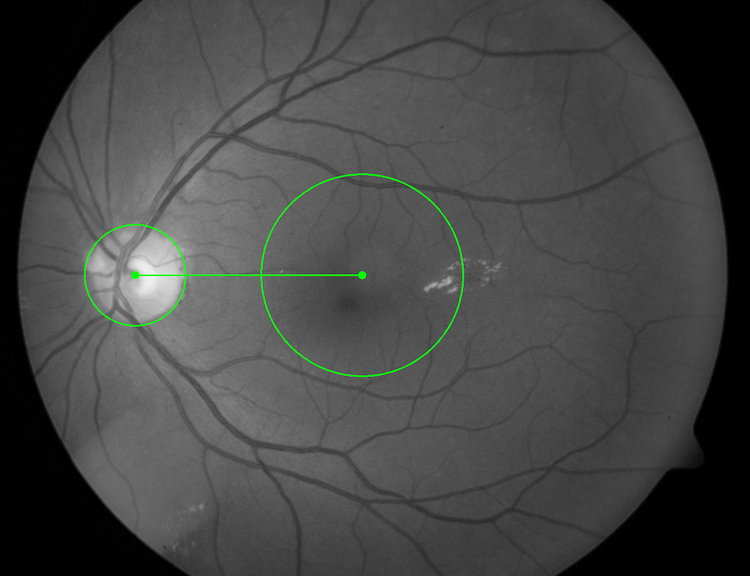
\includegraphics[width=\linewidth]{chap05_fovea_shift}
    \caption{Extrahovaný zelený kanál.}
    \label{pic:chap05_fovea_shift}
  \end{minipage}
  \hfill
  \begin{minipage}[c]{0.315\textwidth}
    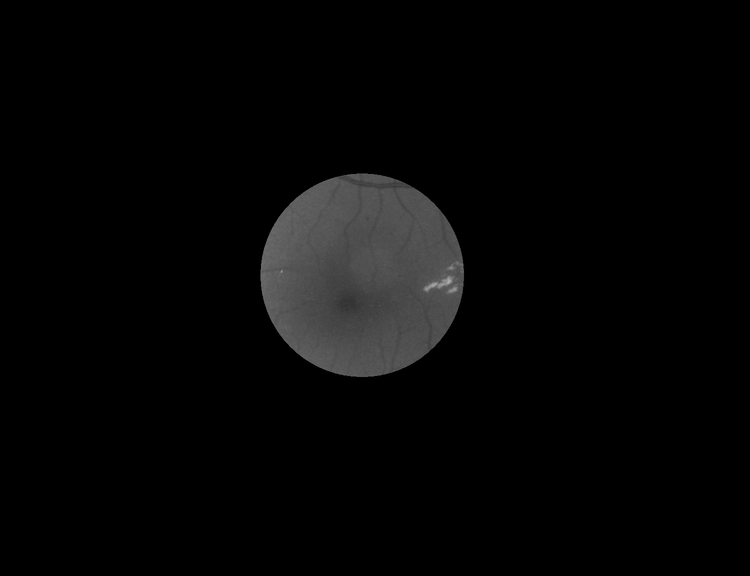
\includegraphics[width=\linewidth]{chap05_fovea_area}
    \caption{Vymezená oblast fovey.}
    \label{pic:chap05_fovea_area}
  \end{minipage}
    \hfill
  \begin{minipage}[c]{0.315\textwidth}
    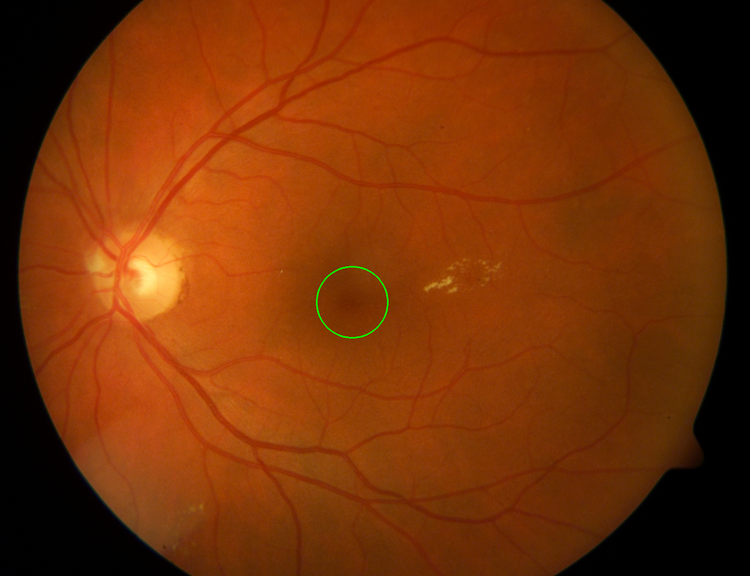
\includegraphics[width=\linewidth]{chap05_fovea_result}
    \caption{Výsledek detekce.}
    \label{pic:chap05_fovea_result}
  \end{minipage}
\end{figure}

\section{Detekce krevního řečiště}
Při detekci příznaků onemocnění na sítnici občas docházelo k~problému, kdy se některé části krevního řečiště jevily jako nález. Důvodem byla velikost dané cévy, její tvar, intenzita ve špatně osvětlených snímcích nebo při rozsáhlém poškození sítnice. Prvotním opatřením byla dodatečná kontrola, zdali se nejedná o~část krevního řečiště. Ta však nebyla příliš úspěšná, protože i přes to, že určitou část chybně detekovaných nálezů vyřadila, stále jich velké množství zůstalo. S~touto nízkou úspěšností bylo potřeba hledat řešení jinde. Velmi dobrých výsledků oproti předchozímu postupu bylo dosaženo při detekci krevního řečiště sítnice a jeho vyloučení ze získaných výsledků.

Jako první se na výchozí snímek (obrázek \ref{pic:chap05_blood_vessels_default}) aplikuje maska pozadí, která vyřadí oblast mimo našeho zájmu, a následně se extrahuje zelený kanál. Jak již bylo zmíněno, na zeleném kanále lze velmi dobře vidět kontrast pozadí sítnice a struktur nacházejících se na ní včetně krevního řečiště (viz obrázek \ref{pic:chap05_blood_vessels_green}). Na tento kanál se aplikuje Gaussovo adaptivní prahování, které transformuje obraz ve stupních šedi na binární obraz. Prahová hodnota se vypočítává jednotlivě pro každý pixel, kde se tento výpočet získá váženým součtem sousedních pixelů daného pixelu, od kterého se odečte určitá konstanta. Ta spolu s~velikostí okolí každého pixelu představuje parametry Gaussova adaptivního prahování. Čím je toto okolí menší, tím je tato metoda citlivější na drobné útvary a naopak čím je okolí větší, tím se tyto drobné útvary z~výsledku ztrácejí. Pokud je okolí pixelů příliš malé, do výsledků se začnou zahrnovat i oblasti, které nenáleží krevnímu řečišti a které mohou obsahovat i případné nálezy. Důležité tedy je zvolit velikost okolí tak, aby byl výsledek dostatečně podrobný a zároveň aby se nepřišlo o~příliš velké množství správných oblastí. Po experimentování s~různými snímky jsem tyto parametry zvolil 49 pro velikost okolí a 3 pro odečítanou konstantu. S~těmito hodnotami bylo dosaženo nejlepších výsledků (obrázek \ref{pic:chap05_blood_vessels_thresh}).

\begin{figure}[h]
  \begin{minipage}[c]{0.315\textwidth}
    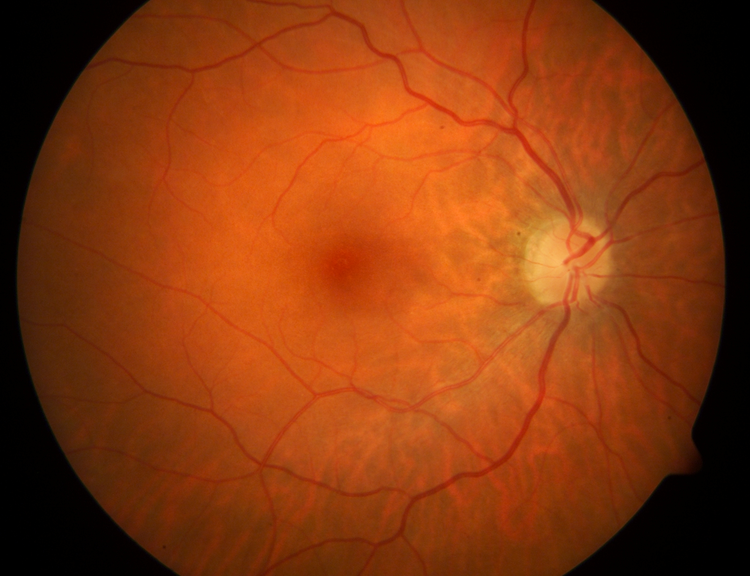
\includegraphics[width=\linewidth]{chap05_blood_vessels_default}
    \caption{Výchozí snímek sítnice.}
    \label{pic:chap05_blood_vessels_default}
  \end{minipage}
  \hfill
  \begin{minipage}[c]{0.315\textwidth}
    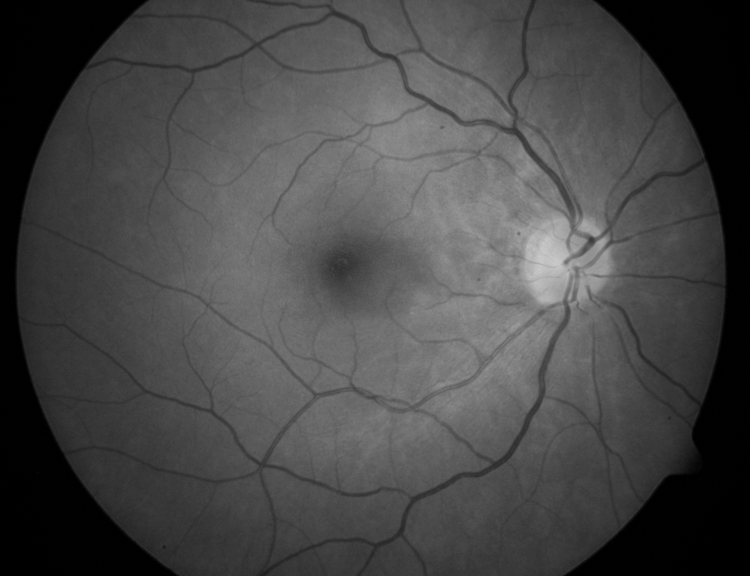
\includegraphics[width=\linewidth]{chap05_blood_vessels_green}
    \caption{Extrahovaný zelený kanál.}
    \label{pic:chap05_blood_vessels_green}
  \end{minipage}
  \hfill
  \begin{minipage}[c]{0.315\textwidth}
    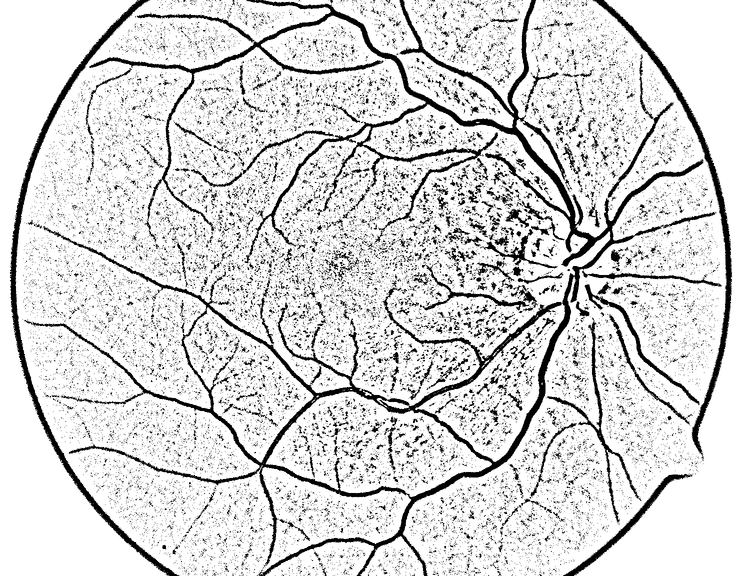
\includegraphics[width=\linewidth]{chap05_blood_vessels_thresh}
    \caption{Gaussovo adaptivní prahování.}
    \label{pic:chap05_blood_vessels_thresh}
  \end{minipage}
\end{figure}

Výstup prahování obsahuje i hraniční oblast mezi sítnicí a pozadím snímku, která byla nesprávně detekována. Této oblasti se zbavíme opětovným aplikováním masky pozadí. Nejprve se však snímek invertuje, protože to vyžaduje další zpracování, a pokud by se maska aplikovala jako první, došlo by i k~jejímu invertování a následně by se musela aplikovat znovu. Samotná maska se musí před jejím použitím upravit, protože hraniční oblast v~některých případech lehce zasahuje do oblasti sítnice. Aby se odstranila i tato přesahující část, provede se eroze sítnice v~masce. Výsledek tohoto zpracování lze vidět na obrázku \ref{pic:chap05_blood_vessels_inverted}.
Nyní následuje mediánové vyhlazování s~velikostí matice 5$\times$5, které redukuje šum typu sůl a pepř (viz sekce \ref{sec:smoothing}). Výsledný obraz ještě jednou podstoupí toto vyhlazování se stejnou maticí. To pomůže k~další redukci nežádoucích oblastí ze snímku (viz obrázek \ref{pic:chap05_blood_vessels_median}). 

\begin{figure}[h]
  \begin{minipage}[c]{0.47\textwidth}
    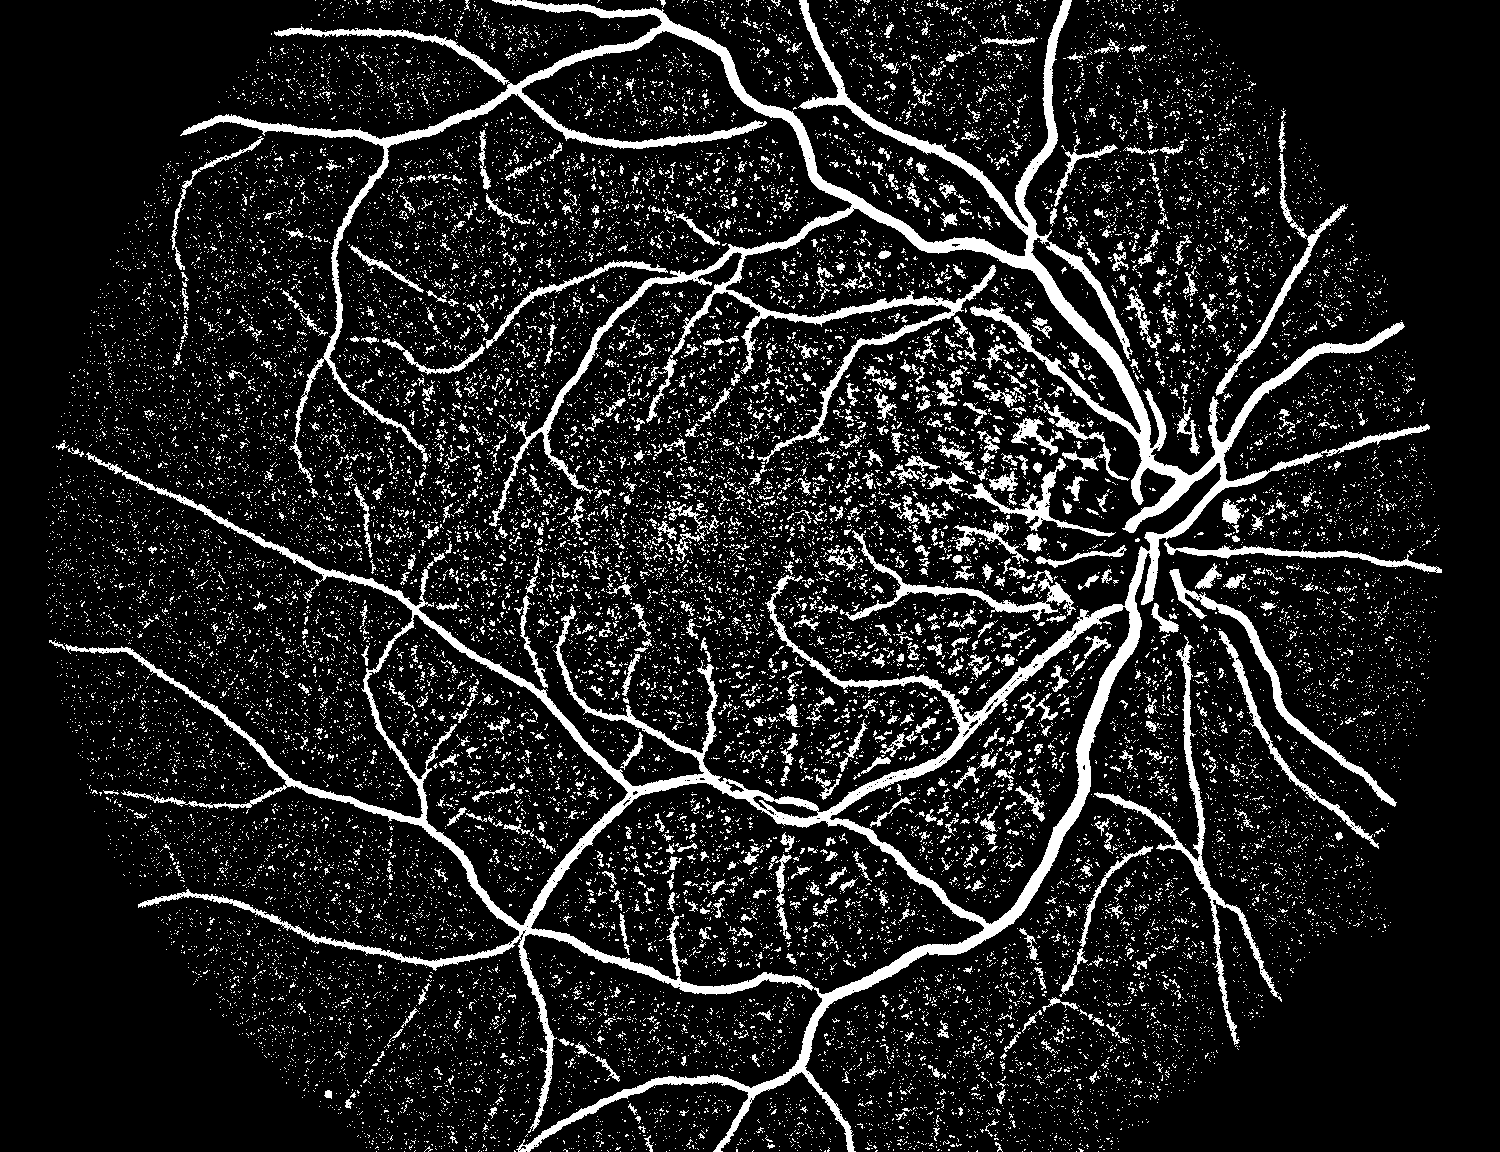
\includegraphics[width=\linewidth]{chap05_blood_vessels_inverted}
    \caption{Invertovaný výstup prahování.}
    \label{pic:chap05_blood_vessels_inverted}
  \end{minipage}
  \hfill
  \begin{minipage}[c]{0.47\textwidth}
    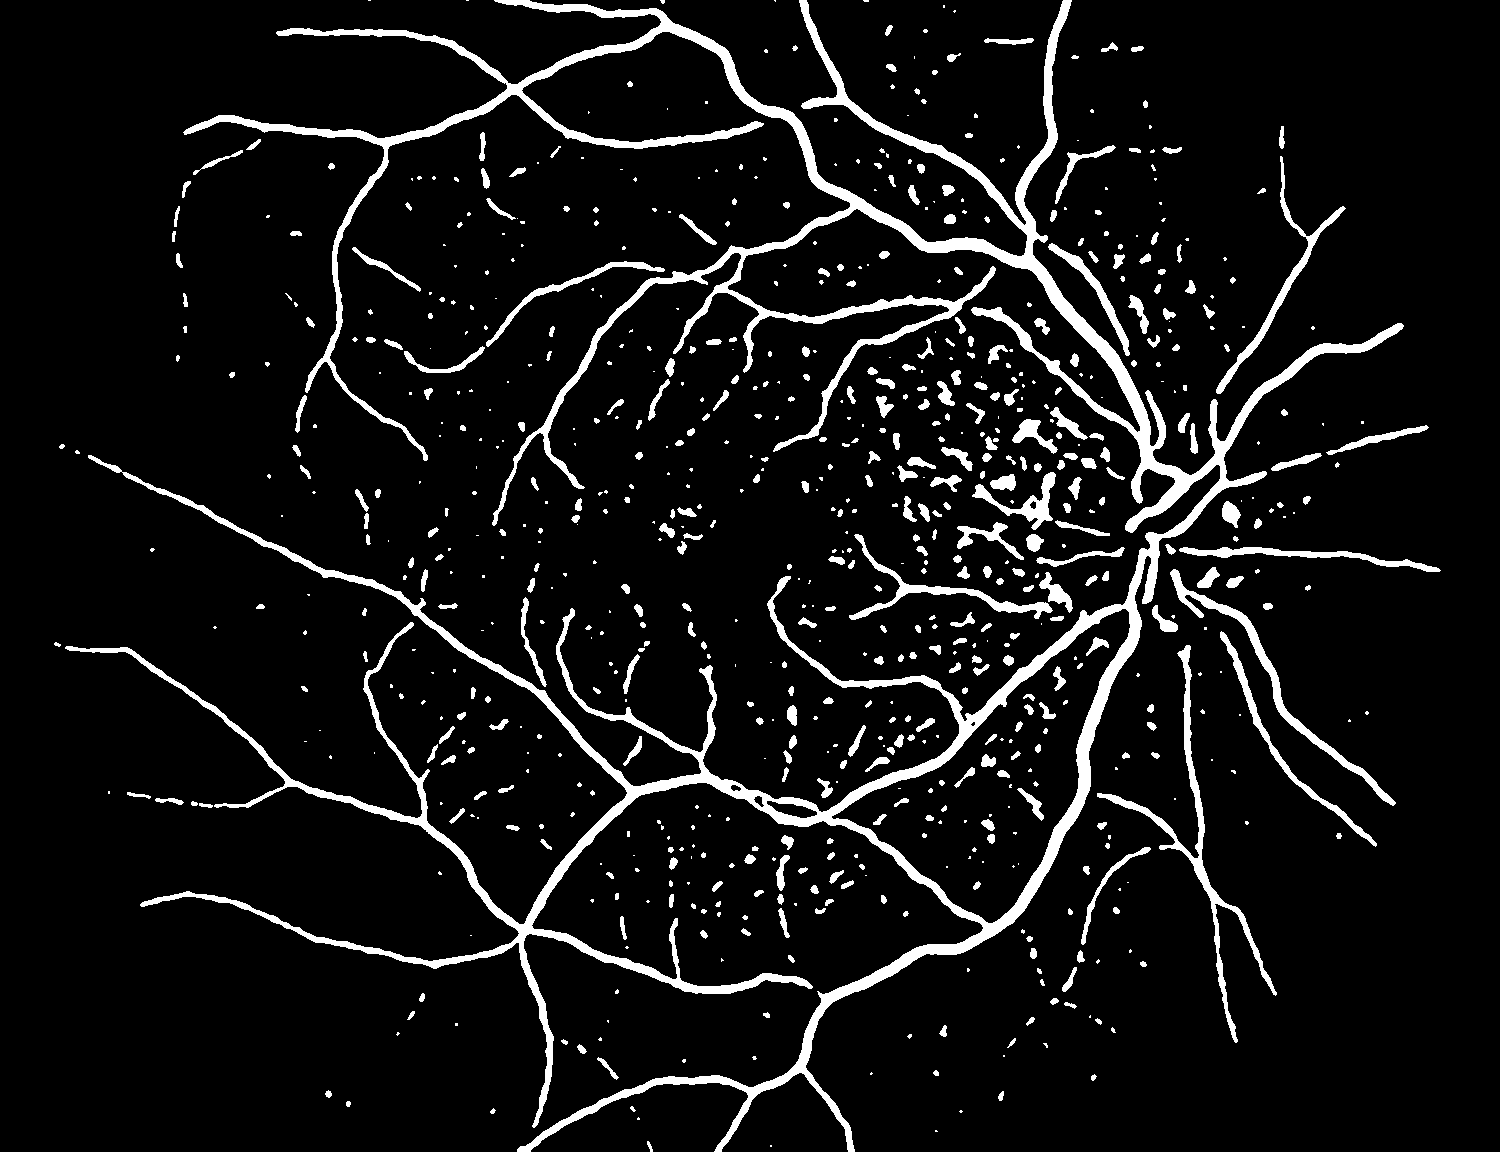
\includegraphics[width=\linewidth]{chap05_blood_vessels_median}
    \caption{Druhé mediánové vyhlazování.}
    \label{pic:chap05_blood_vessels_median}
  \end{minipage}
\end{figure}

Pro získání výsledné masky krevního řečiště se využívá semínkového vyplňování začínající na cévách v~optickém disku. Z~tohoto důvodu je potřeba vypočítat množinu počátečních bodů (semínek) a k~tomu jsou použity parametry optického disku, který byl již detekován. Nejprve se vytvoří nová maska obsahující kružnici kolem optického disku, která se následně bitově vynásobí výstupem z~Gaussova adaptivního prahování. Na nově získané masce se nyní pomocí Houghovy transformace detekují přímky. V~oblasti optického disku mají cévy největší průměr, proto se této vlastnosti využije při hledání těchto přímek specifikováním jejich minimální délky. Nyní už je na řadě semínkové vyplňování, u~kterého se jako počáteční body využijí středy detekovaných přímek. Výsledek po této operaci je viditelný na obrázku \ref{pic:chap05_blood_vessels_flood_fill}.

Při adaptivním prahování a vyhlazování původního snímku v~procesu detekce krevního řečiště může dojít k~porušení spojitosti cév a tím pádem nejsou některé části krevního řečiště zahrnuty ve výsledné masce. Abychom zamezili ztrátám těchto cév, maska (viz obrázek \ref{pic:chap05_blood_vessels_missed}), ze které bylo semínkovým vyplňováním extrahováno krevní řečiště, podstoupí dalšímu zpracování. To zahrnuje nalezení zbylých oblastí a jejich klasifikace, na jejímž základě se rozhodne, zdali se jedná o~část krevního řečiště nebo jiného objektu. První zkoumané kritérium je obsah dané oblasti. Pokud je obsah větší než 4500, vypočítá se poměr stran nejmenšího obdélníku ohraničujícího danou oblast, a pokud je tento poměr větší nebo roven 8, jedná se o~část cévy, jinak se zahazuje. Pokud je obsah větší než 1600, ponechávají se oblasti s~poměrem stran větším než 10, jinak se vypočítá průměrná šířka této oblasti, a pokud je menší než 6,8 (což by zhruba odpovídalo šířce cévy), oblast zůstává, jinak se zahazuje. Pokud je obsah větší než 300, opět se vypočítá poměr stran pro danou oblast, a pokud je větší nebo roven 5, jedná se o~součást cévy, jinak se zahazuje. Ostatní oblasti s~obsahem menším než 300 se zahazují. Celkový výsledek detekce krevního řečiště je zobrazen na obrázku \ref{pic:chap05_blood_vessels_result}.

\begin{figure}[h]
  \begin{minipage}[c]{0.315\textwidth}
    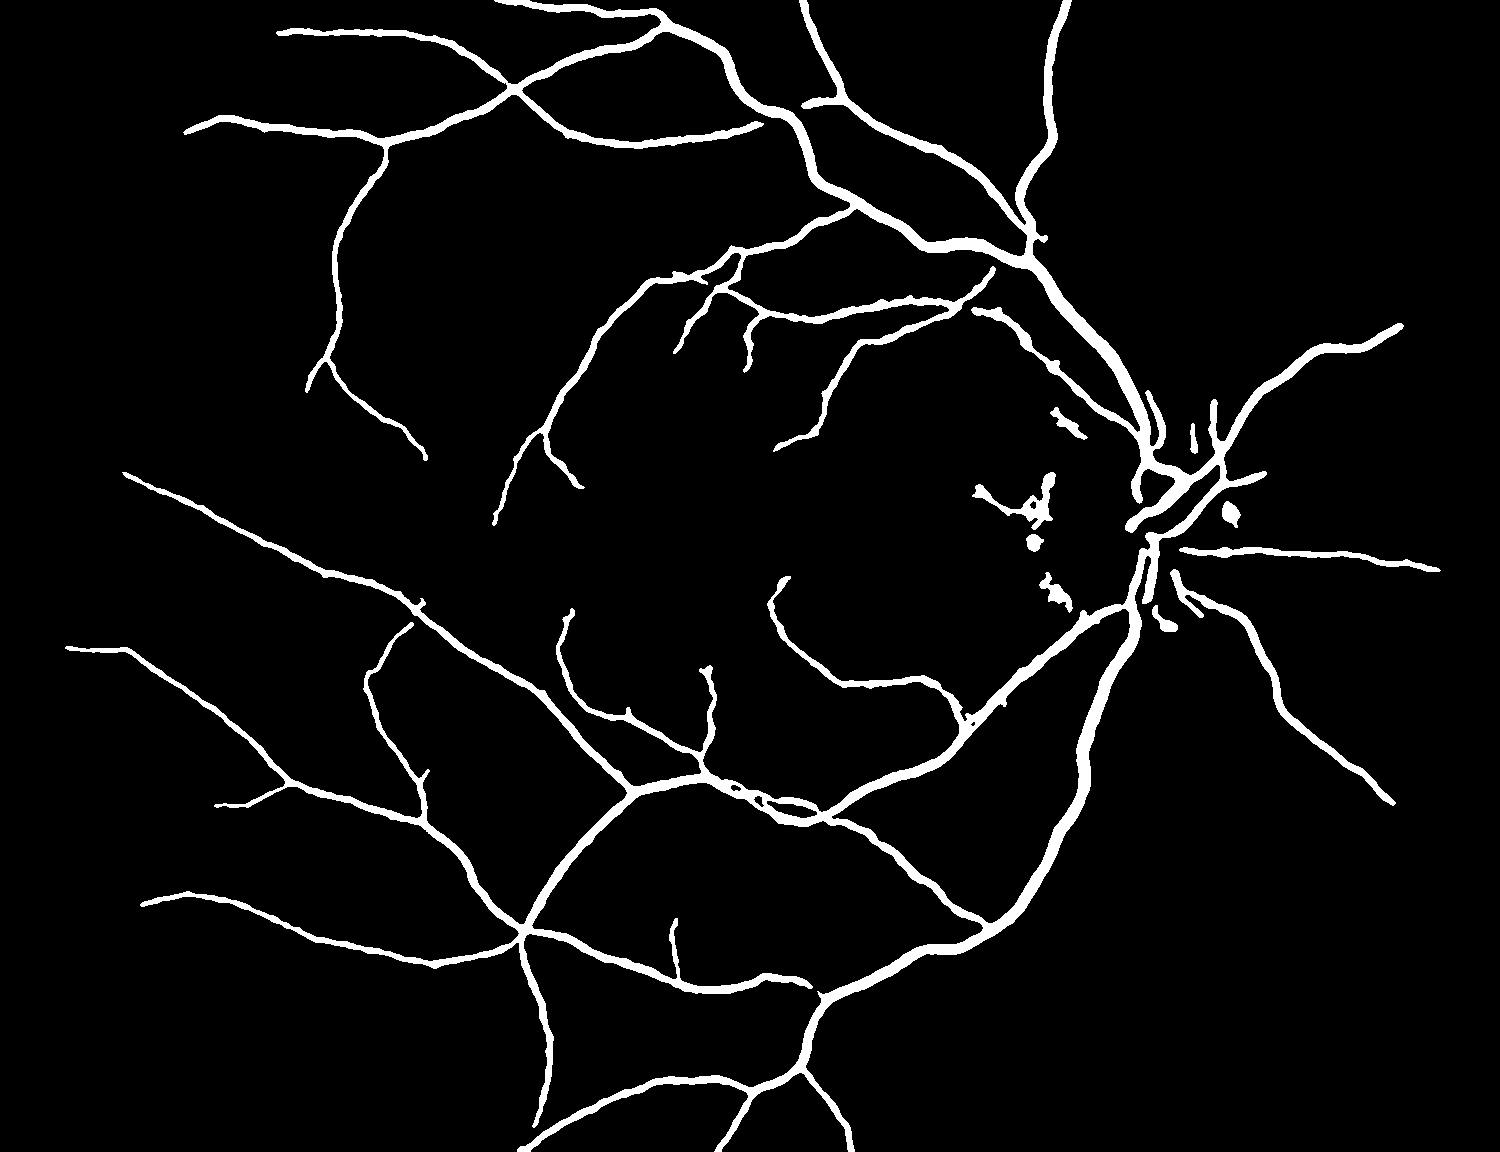
\includegraphics[width=\linewidth]{chap05_blood_vessels_flood_fill}
    \caption{Výsledek semínkového vyplňování.}
    \label{pic:chap05_blood_vessels_flood_fill}
  \end{minipage}
  \hfill
    \begin{minipage}[c]{0.315\textwidth}
    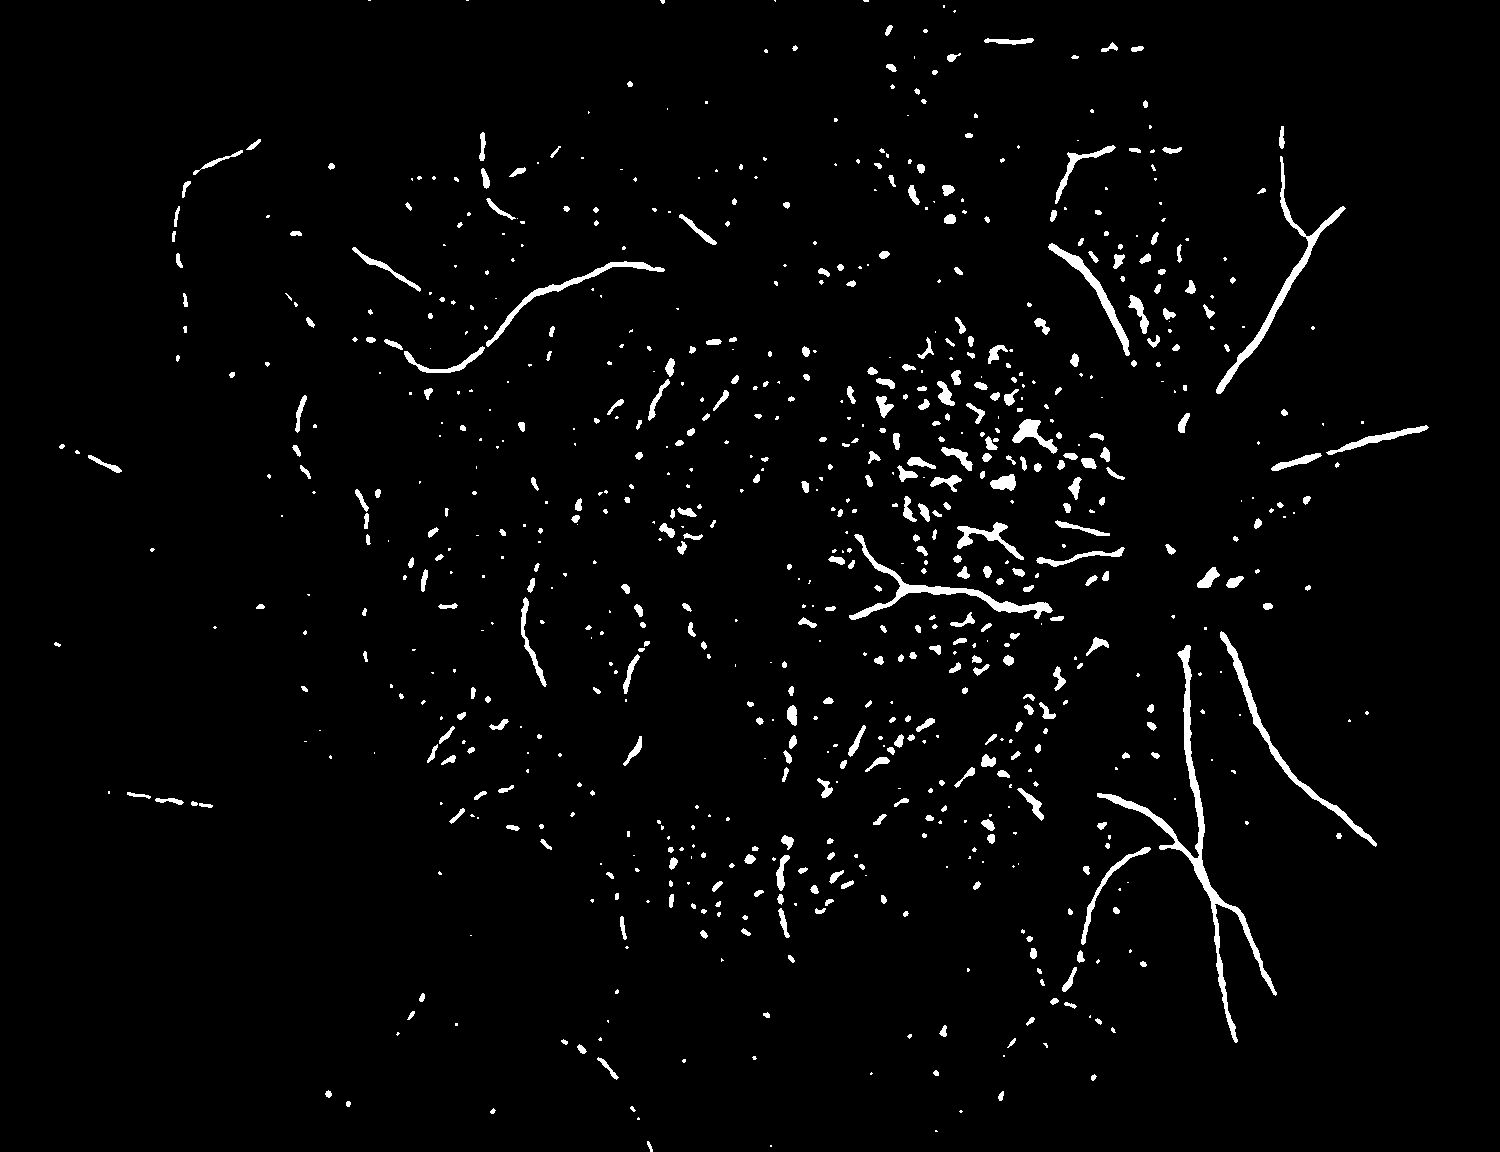
\includegraphics[width=\linewidth]{chap05_blood_vessels_missed}
    \caption{Maska s~vynechanými cévami.}
    \label{pic:chap05_blood_vessels_missed}
  \end{minipage}
  \hfill
  \begin{minipage}[c]{0.315\textwidth}
    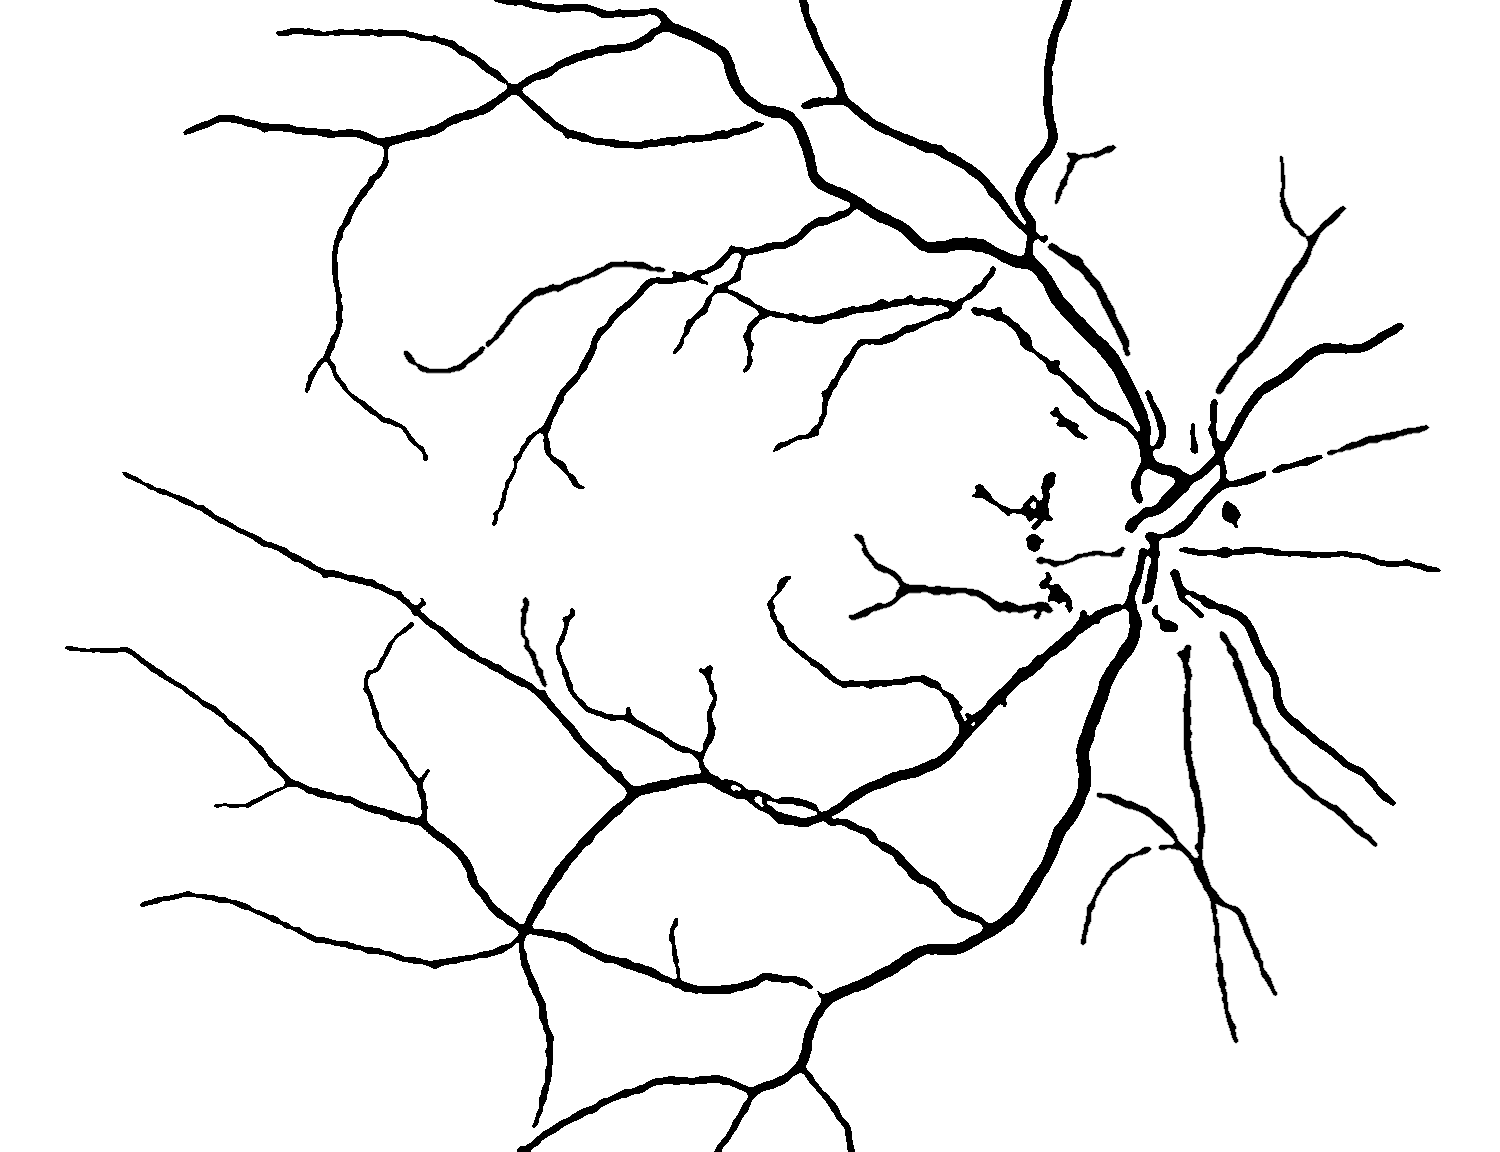
\includegraphics[width=\linewidth]{chap05_blood_vessels_result}
    \caption{Výsledek detekce krevního řečiště.}
    \label{pic:chap05_blood_vessels_result}
  \end{minipage}
\end{figure}


\section{Detekce drúz a exudátů}
Vzhledem k~nedostatku snímků s~VPMD při vytváření této práce se využijí i snímky s~exudáty. Drúzy vznikající při VPMD jsou velmi podobné těmto exudátům, které vznikají při diabetické retinopatii. Z~tohoto důvodu je možné detekovat tyto nálezy stejným algoritmem. V~obou případech se jedná o~tukové látky usazující se na sítnici, které mají žlutou barvu s~vysokou intenzitou. Jejich počet, tvar, velikost a umístění na sítnici se liší u~každého pacienta (viz kapitola \ref{ch:nemoci}).

\subsection*{Vymezení podezřelých oblastí}
Při detekci drúz a exudátů se opět pracuje se zeleným kanálem (obrázek \ref{pic:chap05_disease_green}) výchozího snímku (obrázek \ref{pic:chap05_disease_default}). Na něj je použito normalizované rozmazání s~maskou o~velikosti 7$\times$7~pixelů. Je to z~důvodu, aby se vyloučili drobné nevýrazné oblasti, které jsou někdy obtížné klasifikovat i zkušeným oftalmologem. Nad tímto rozmazaným snímkem se následně provede Gaussovo adaptivní prahování, které je velmi účinné pro vymezení podezřelých oblastí. Jak již bylo zmíněno výše, prahová hodnota u~Gaussova adaptivního prahování se vypočítává jednotlivě pro každý pixel, kde se tento výpočet získá váženým součtem sousedních pixelů daného pixelu, od kterého se odečte určitá konstanta. V~tomto případě je velikost okolí 5~pixelů a odečítaná konstanta je 0, tedy se nic neodečítá. Výsledek tohoto prahování lze vidět na obrázku \ref{pic:chap05_disease_threshold}. Teprve nyní se může aplikovat maska obsahující oblasti krevního řečiště a optického disku, které již byly detekovány dříve. Pokud by tato maska byla použita hned na začátku, nepříznivě by ovlivnila toto prahování, protože by v~obraze vznikl příliš velký kontrast mezi vyloučenými oblastmi a zbylou částí sítnice. To by způsobilo zahrnutí obrysů cév a optického disku do podezřelých oblastí, což je nežádoucí. Po aplikaci masky obraz následně podstoupí mediánovému vyhlazení s~velikostí matice 5$\times$5, aby se z~něj odstranil šum. Výsledné podezřelé oblasti jsou zachyceny na obrázku \ref{pic:chap05_disease_suspect}.

\begin{figure}[h]
  \begin{minipage}[c]{0.47\textwidth}
    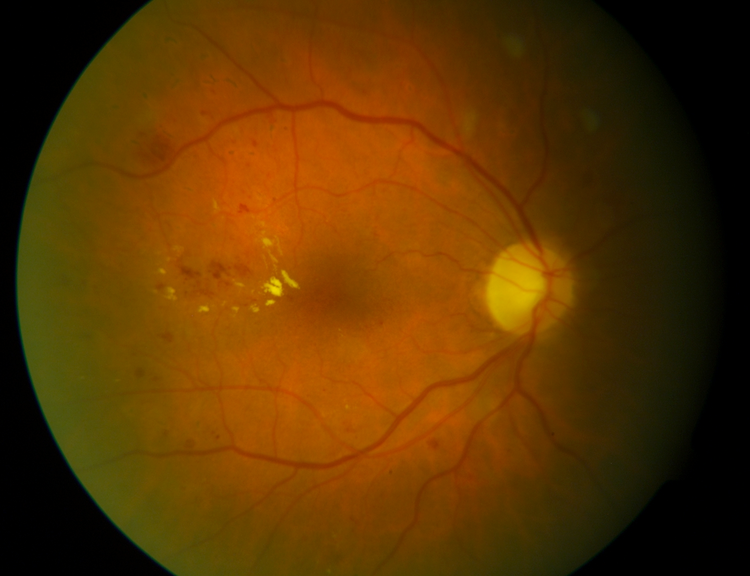
\includegraphics[width=\linewidth]{chap05_disease_default}
    \caption{Výchozí snímek.}
    \label{pic:chap05_disease_default}
  \end{minipage}
  \hfill
  \begin{minipage}[c]{0.47\textwidth}
    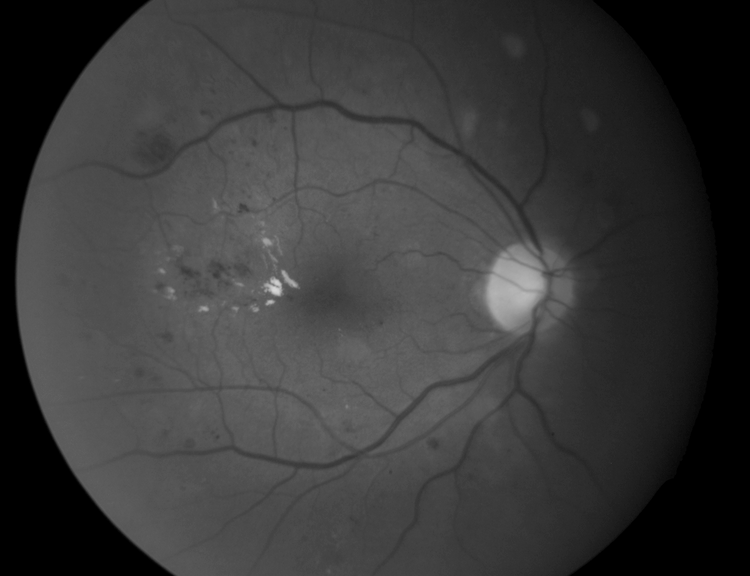
\includegraphics[width=\linewidth]{chap05_disease_green}
    \caption{Extrahovaný zelený kanál.}
    \label{pic:chap05_disease_green}
  \end{minipage}
\end{figure}

\begin{figure}[h]
  \begin{minipage}[c]{0.47\textwidth}
    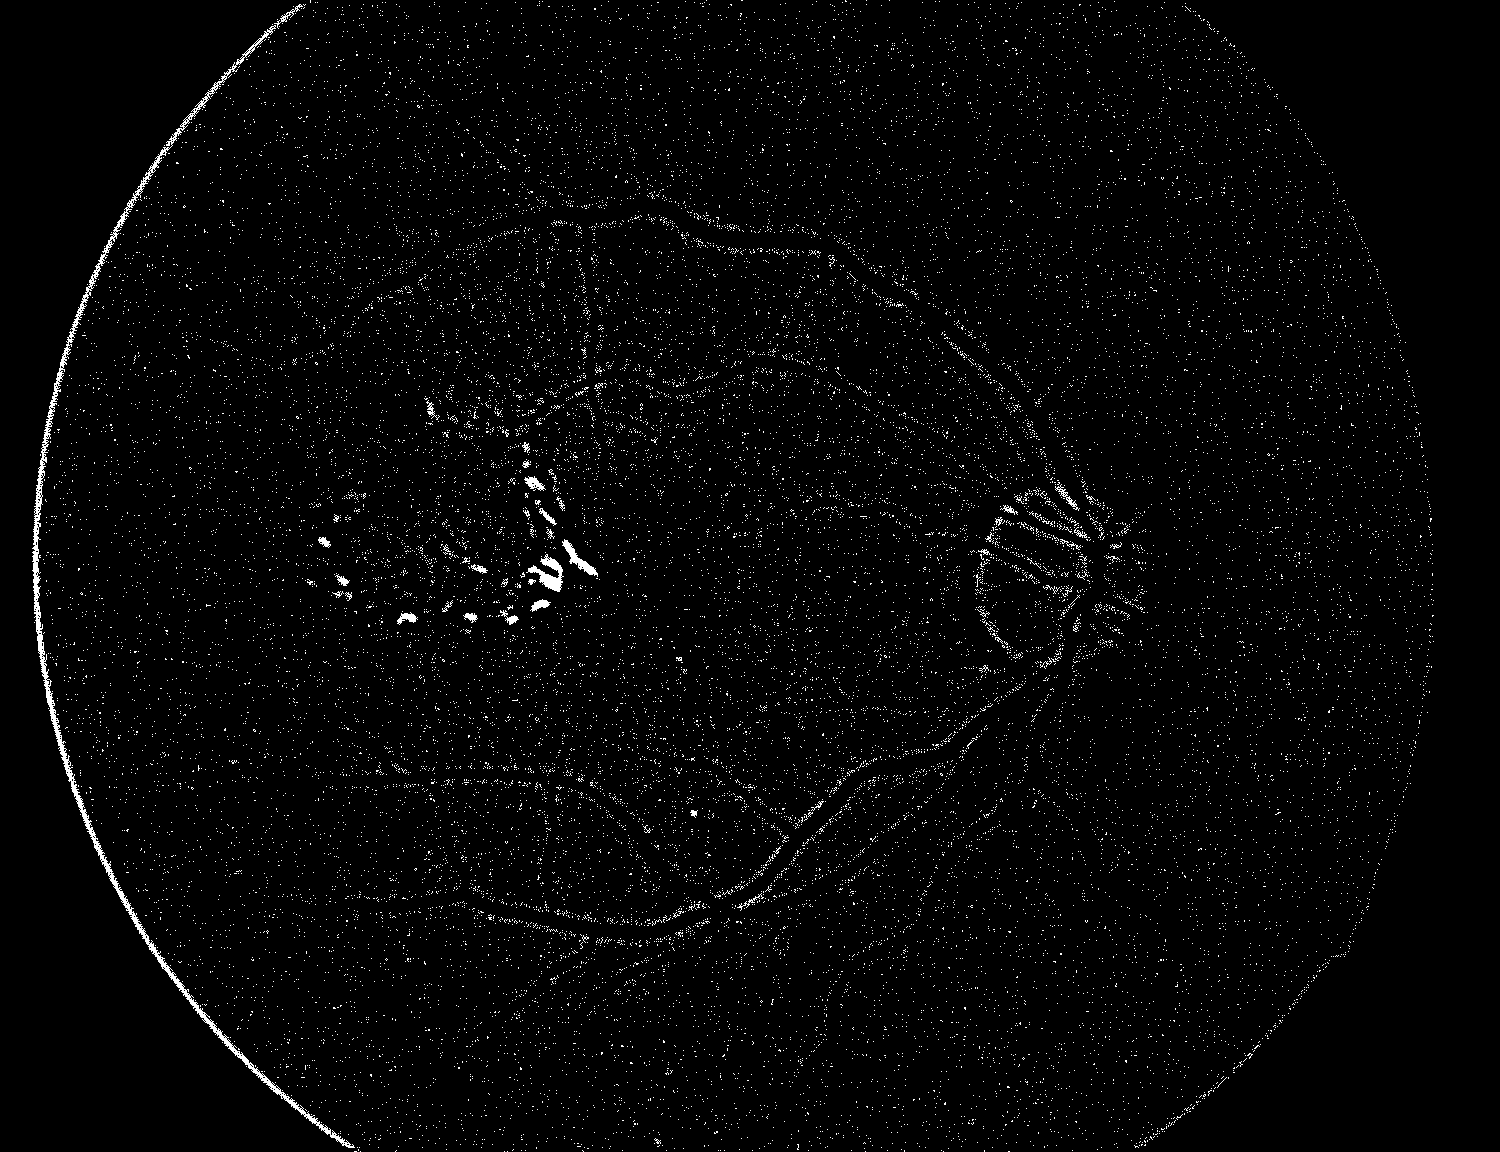
\includegraphics[width=\linewidth]{chap05_disease_threshold}
    \caption{Výsledek prahování.}
    \label{pic:chap05_disease_threshold}
  \end{minipage}
  \hfill
  \begin{minipage}[c]{0.47\textwidth}
    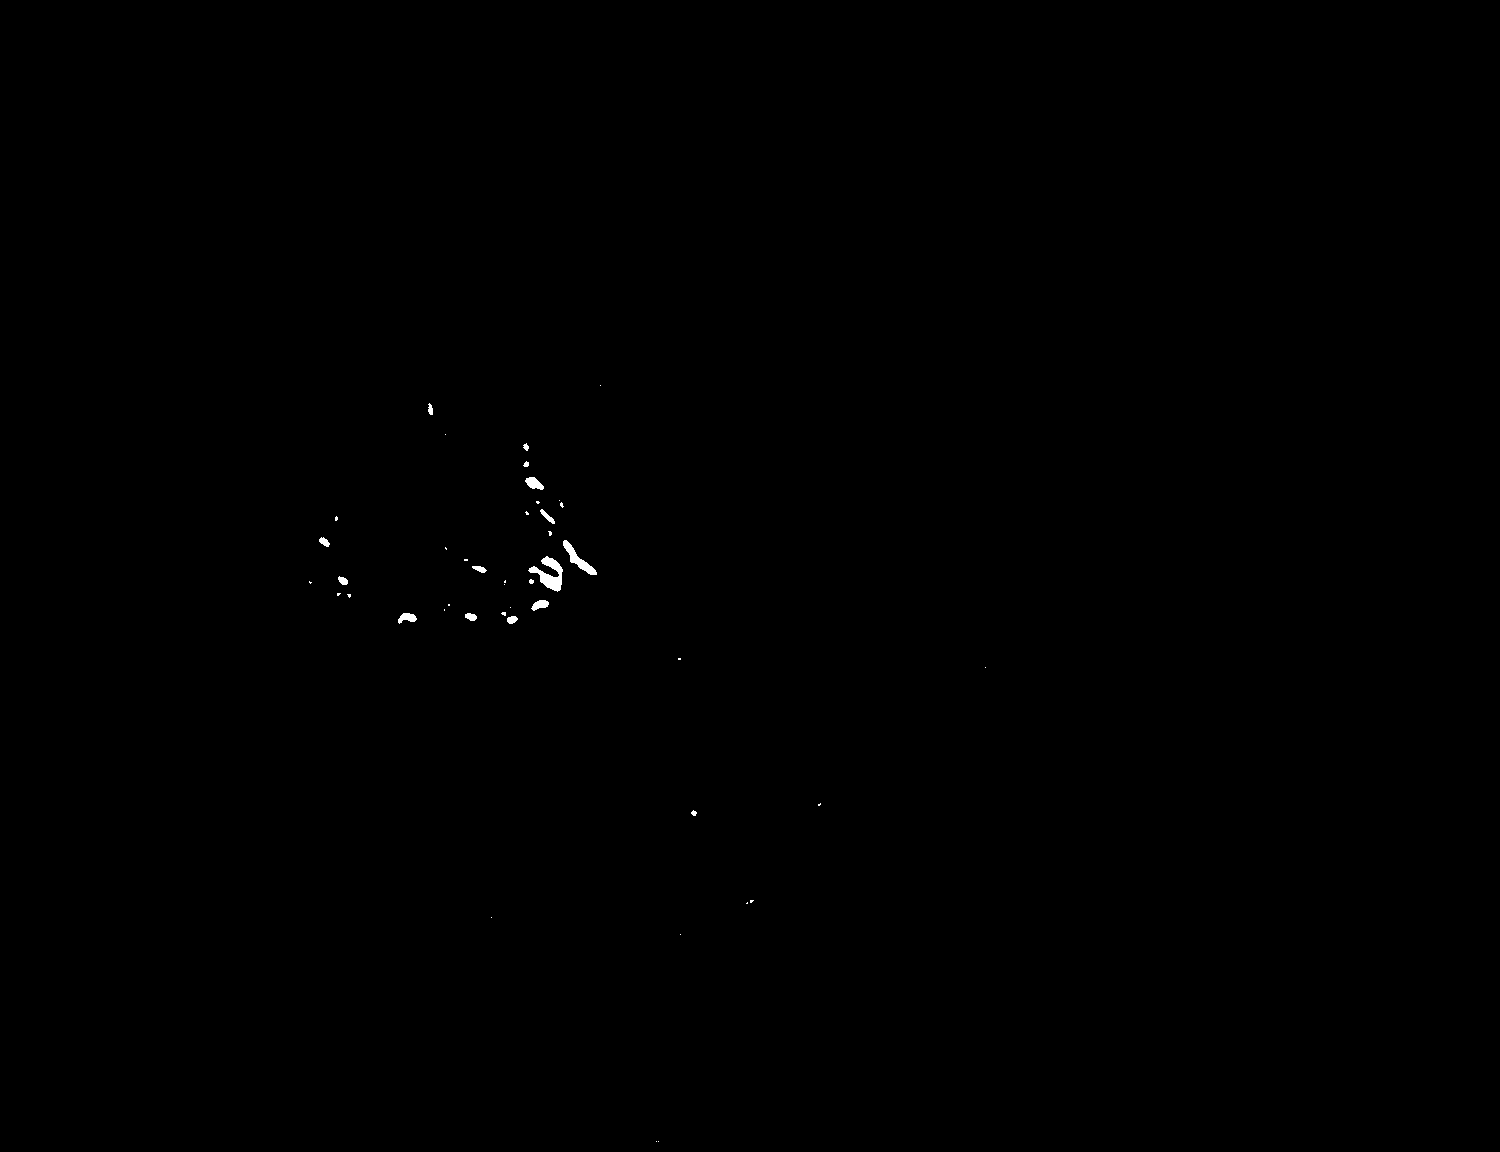
\includegraphics[width=\linewidth]{chap05_disease_suspect}
    \caption{Získané podezřelé oblasti.}
    \label{pic:chap05_disease_suspect}
  \end{minipage}
\end{figure}


\subsection*{Úprava masky krevního řečiště}
Snímky sítnic, jejichž krevní řečiště velmi dobře kontrastuje s~pozadím sítnice, způsobí, že obrysy těchto cév se zahrnou do podezřelých oblastí. Aby se tomu zabránilo, je potřeba provést úpravu masky krevního řečiště ještě před jejím použitím. Úprava představuje dilataci této masky, aby došlo k~rozšíření daných cév. Rozdíl mezi původní a dilatovanou maskou je zobrazen na obrázcích \ref{pic:chap05_disease_vessel_mask} a \ref{pic:chap05_disease_vessel_mask_dilated}. Jakmile se tato maska aplikuje, vyloučí se ze zpracovávaného snímku nežádoucí obrysy. Porovnání mezi podezřelými oblastmi, na nichž se použila neupravená a upravená maska, lze vidět na obrázcích \ref{pic:chap05_disease_suspect_unchanged} a \ref{pic:chap05_disease_suspect_changed}.

\begin{figure}[h]
  \begin{minipage}[c]{0.47\textwidth}
    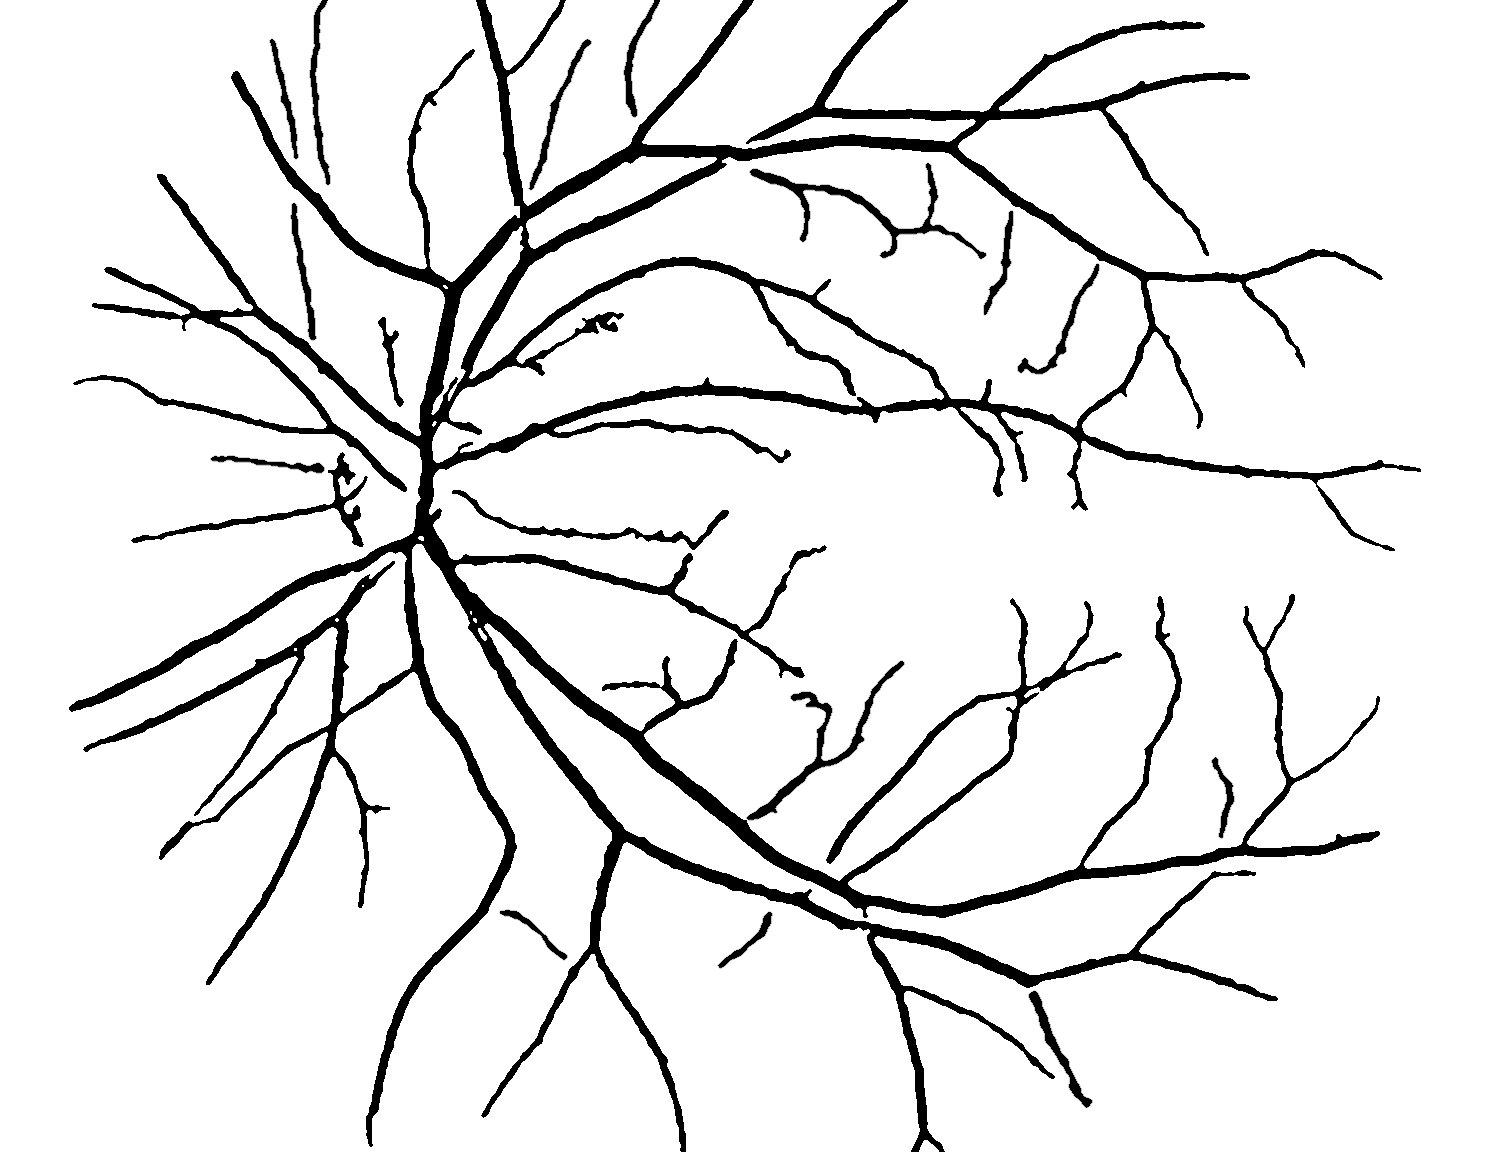
\includegraphics[width=\linewidth]{chap05_disease_vessel_mask}
    \caption{Původní maska.}
    \label{pic:chap05_disease_vessel_mask}
  \end{minipage}
  \hfill
  \begin{minipage}[c]{0.47\textwidth}
    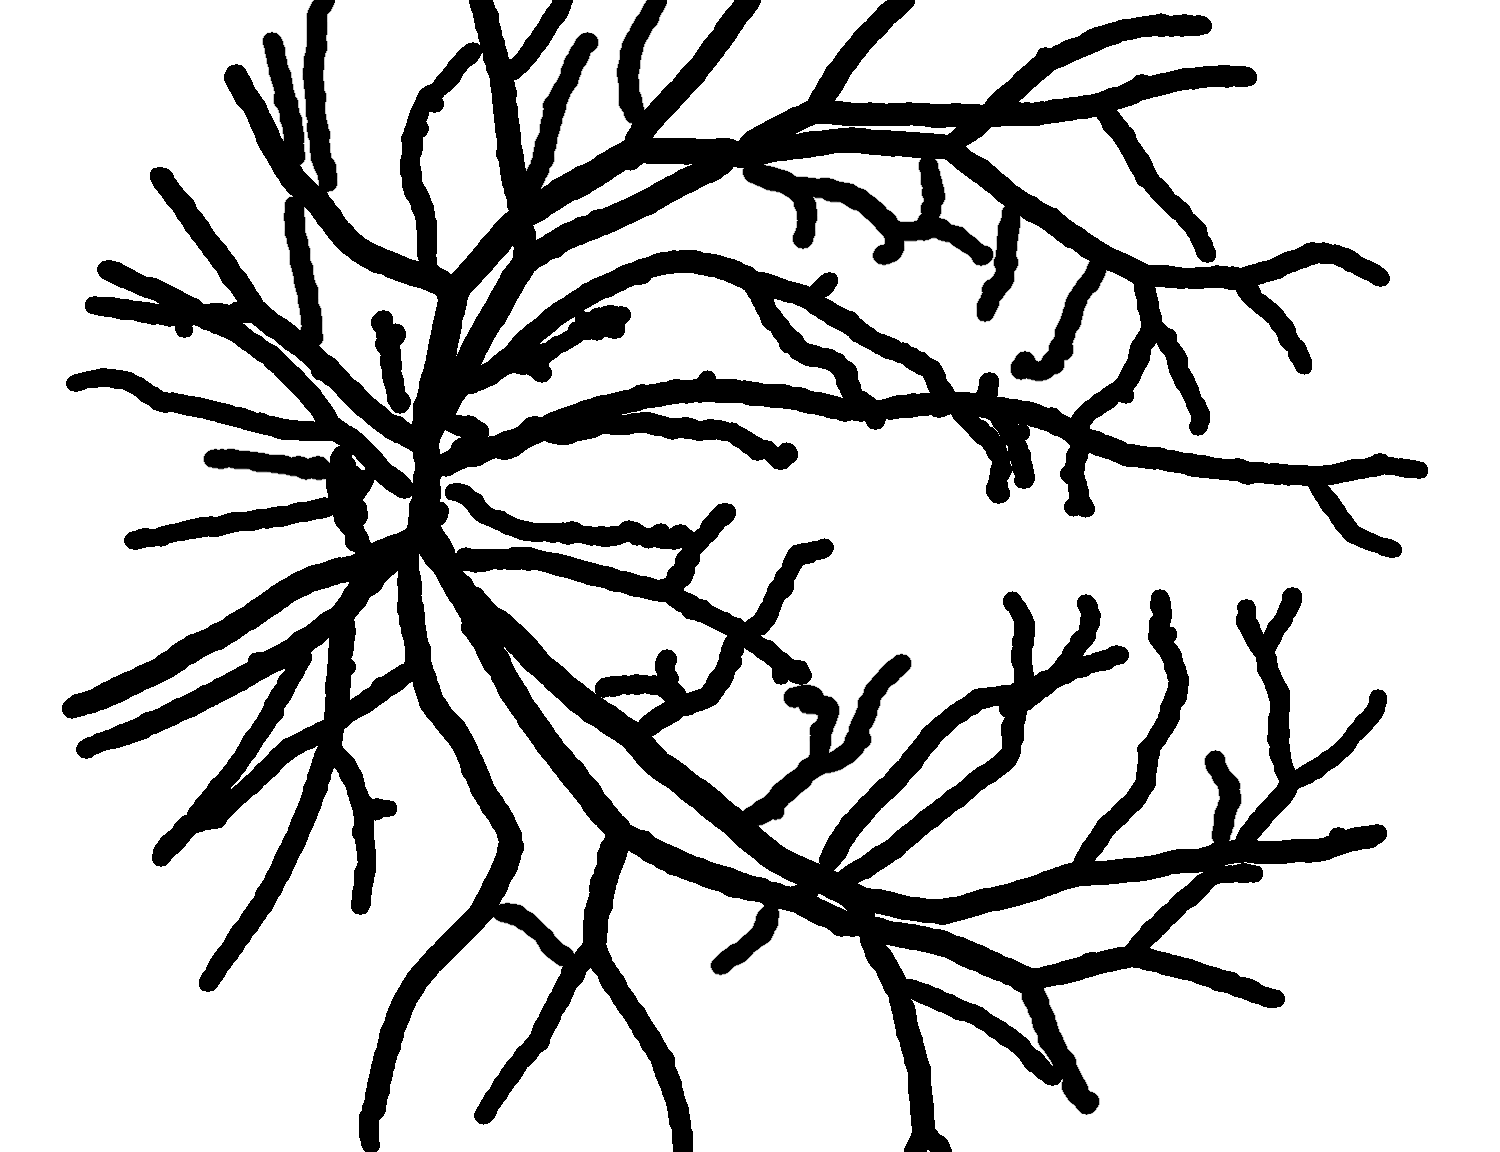
\includegraphics[width=\linewidth]{chap05_disease_vessel_mask_dilated}
    \caption{Maska po dilataci.}
    \label{pic:chap05_disease_vessel_mask_dilated}
  \end{minipage}
\end{figure}

\begin{figure}[h]
  \begin{minipage}[c]{0.47\textwidth}
    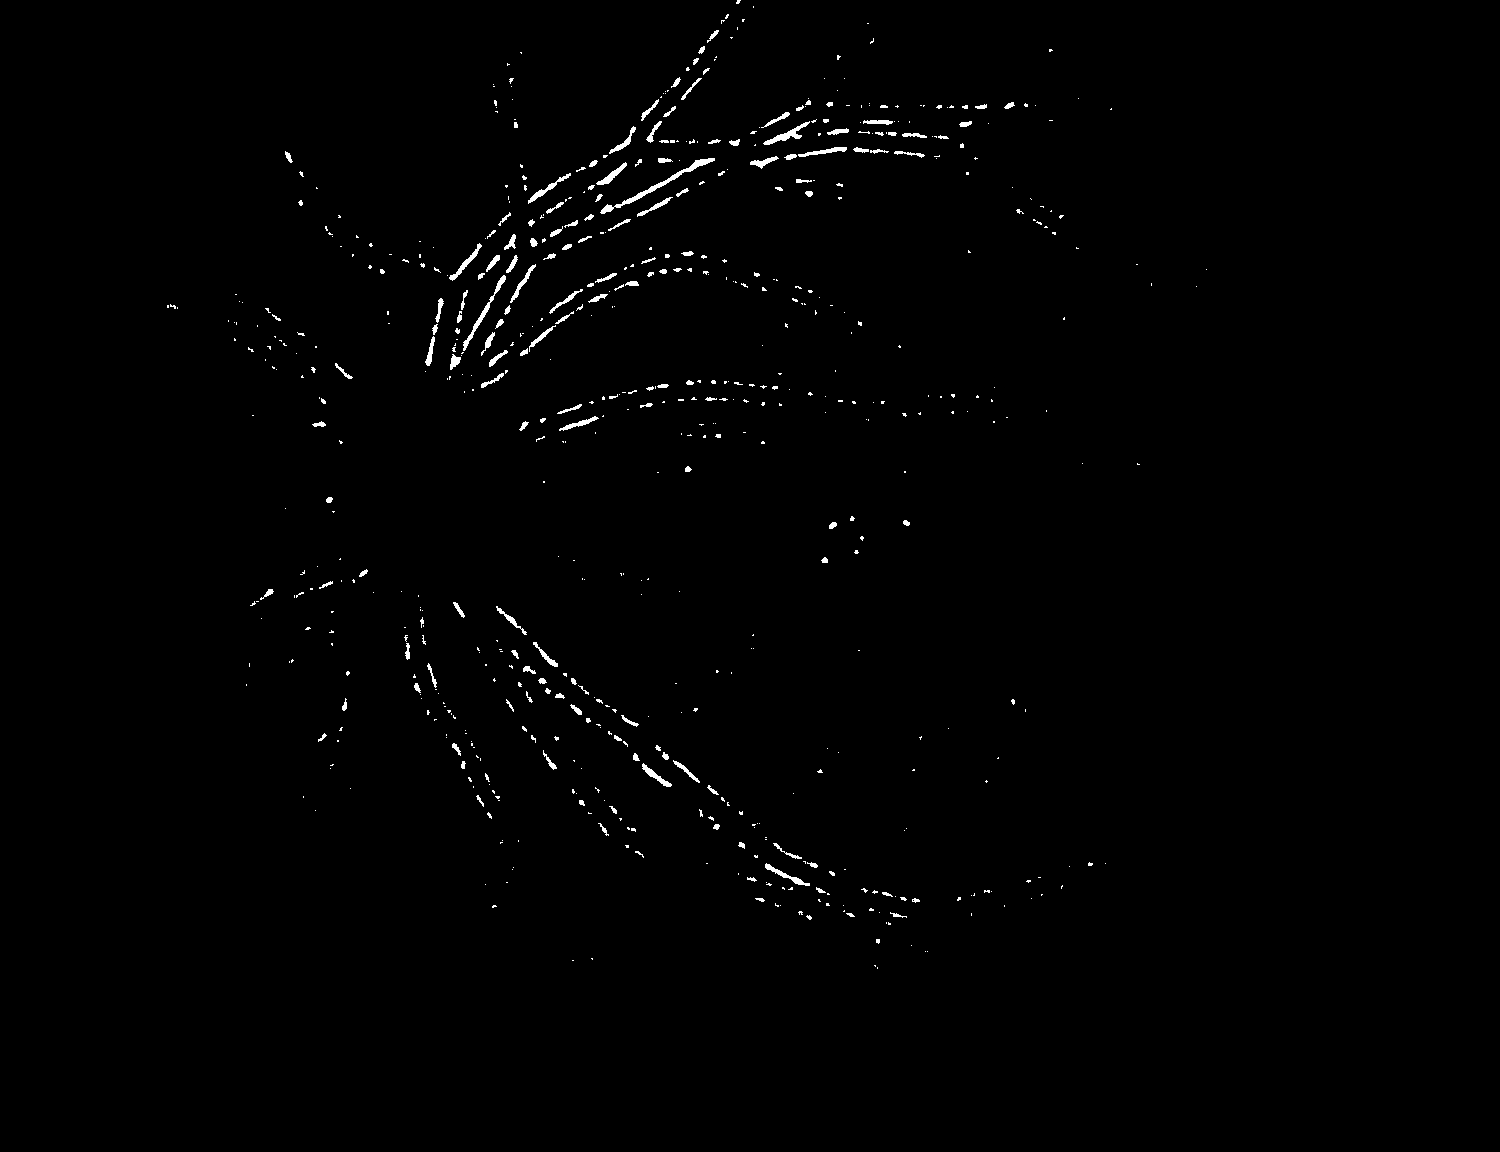
\includegraphics[width=\linewidth]{chap05_disease_suspect_unchanged}
    \caption{Podezřelé oblasti s~neupravenou maskou.}
    \label{pic:chap05_disease_suspect_unchanged}
  \end{minipage}
  \hfill
  \begin{minipage}[c]{0.47\textwidth}
    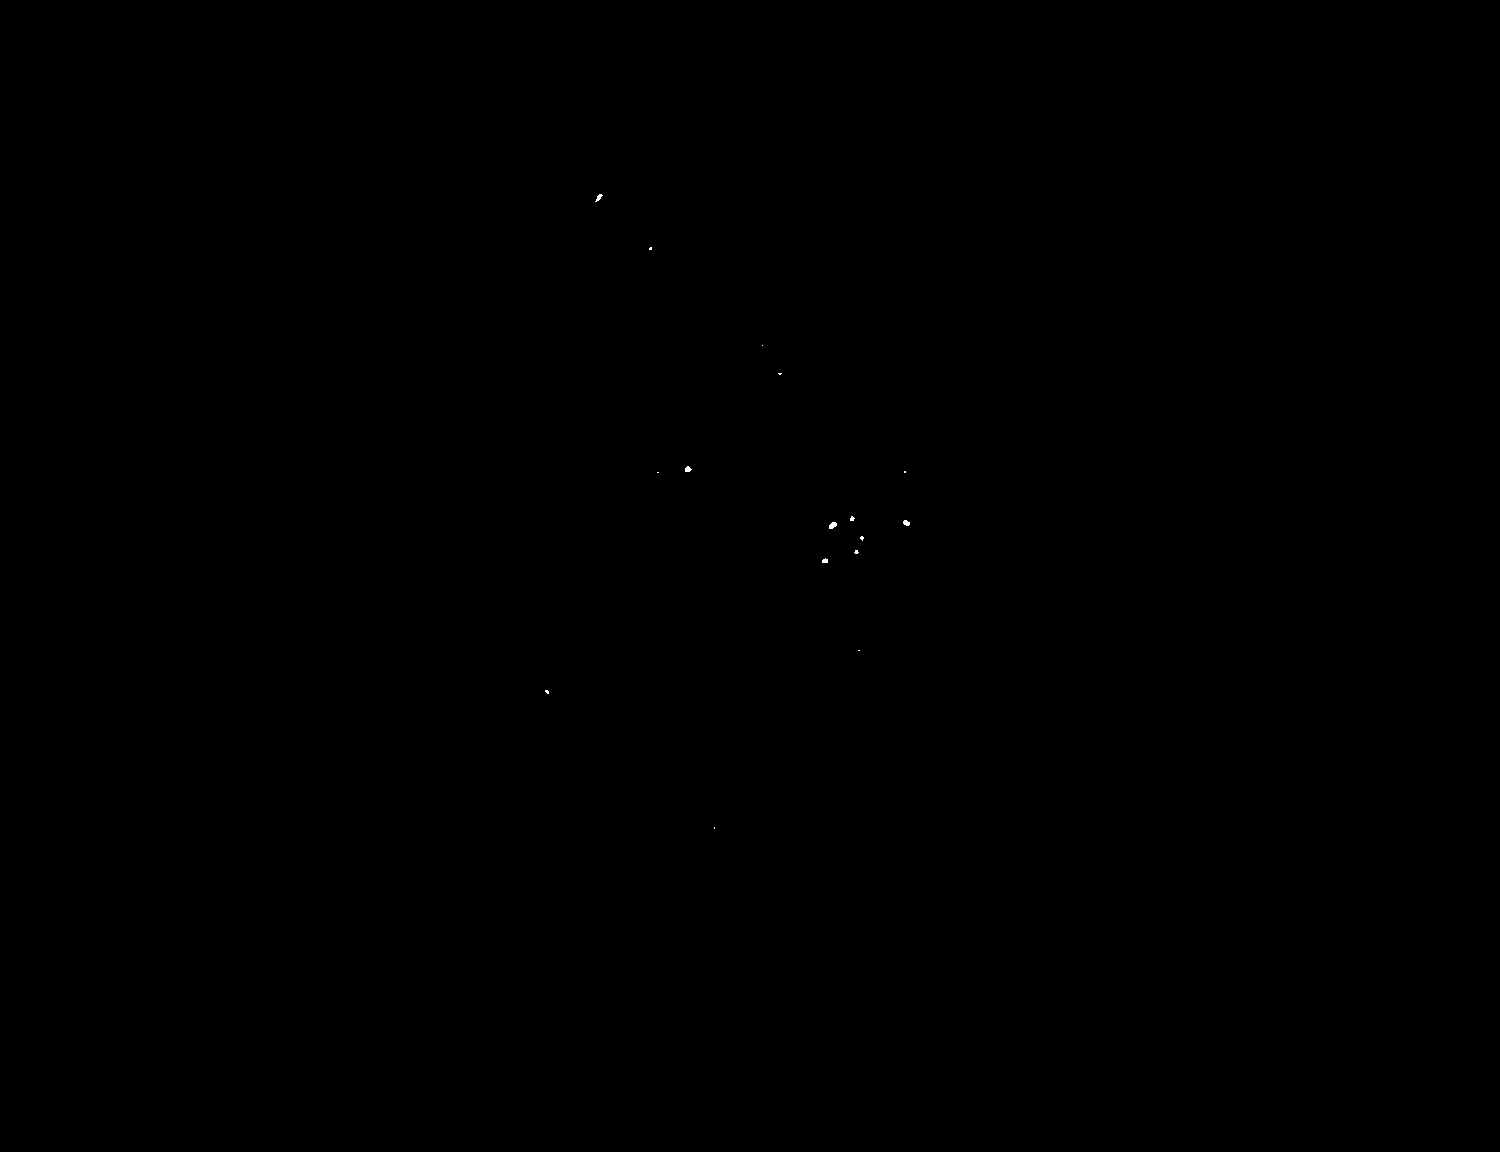
\includegraphics[width=\linewidth]{chap05_disease_suspect_changed}
    \caption{Podezřelé oblasti s~upravenou maskou.}
    \label{pic:chap05_disease_suspect_changed}
  \end{minipage}
\end{figure}


\subsection*{Klasifikace podezřelých oblastí}
Posledním krokem je určit, které z~vymezených podezřelých oblastí představují drúzy či exudáty a které naopak ne. K~tomuto účelu se využívá HSV barevného modelu, do kterého je vstupní snímek převeden. HSV barevný model se skládá ze tří složek, kterými jsou: barevný tón (hue), sytost barvy (saturation) a hodnota jasu (value) neboli množství bílého světla v~obraze.

Nejprve se naleznou obrysy podezřelých oblastí, na jejichž základě se vypočítají jejich obsahy. Pokud je obsah dané plochy větší než 3~pixely, lokalizuje se odpovídající plocha v~HSV obrázku. Z~toho lze následně vypočítat průměrnou hodnotu barevného tónu, sytost a jas této oblasti. Experimentováním nad různými obrázky byly vytyčeny meze, které jsou uvedeny v~tabulce \ref{tab:hsv_color_limits}. Pokud některá z~oblastí spadá do jedné z~těchto mezí, jedná se o~drúzu nebo exudát.

\begin{table}[ht]
  \begin{center}	
    \begin{tabular}{|c|c|c|c|}
      \hline
      Hodnota & Mez 1 & Mez 2   & Mez 3 \\
      \hline
      H & 30--12   &  30--15 &  30--19 \\
      \hline
      S~& 255--170 & 255--120 & 255--187 \\
      \hline
      V~& 255--120 & 255--84 & 255--75 \\
      \hline
    \end{tabular}
  \caption{Přehled HSV mezí pro klasifikaci podezřelých oblastí.}
  \label{tab:hsv_color_limits}
  \end{center}
\end{table}

Jakmile byla oblast klasifikována jako nález, vypočítá se pomocí matematických momentů její těžiště, které představuje střed, ze kterého se vytvoří kružnice pro označení nálezu. Značení se nejprve provádí do prázdného snímku, ze kterého jsou po zkontrolování všech oblastí vybrány externí obrysy. Ty jsou zakresleny do výsledného obrázku, aby jednotlivé kružnice nepřekrývaly detekované nálezy. Výsledek detekce lze vidět na obrázku \ref{pic:chap05_disease_result}.

\begin{figure}[h]
  \begin{center}
    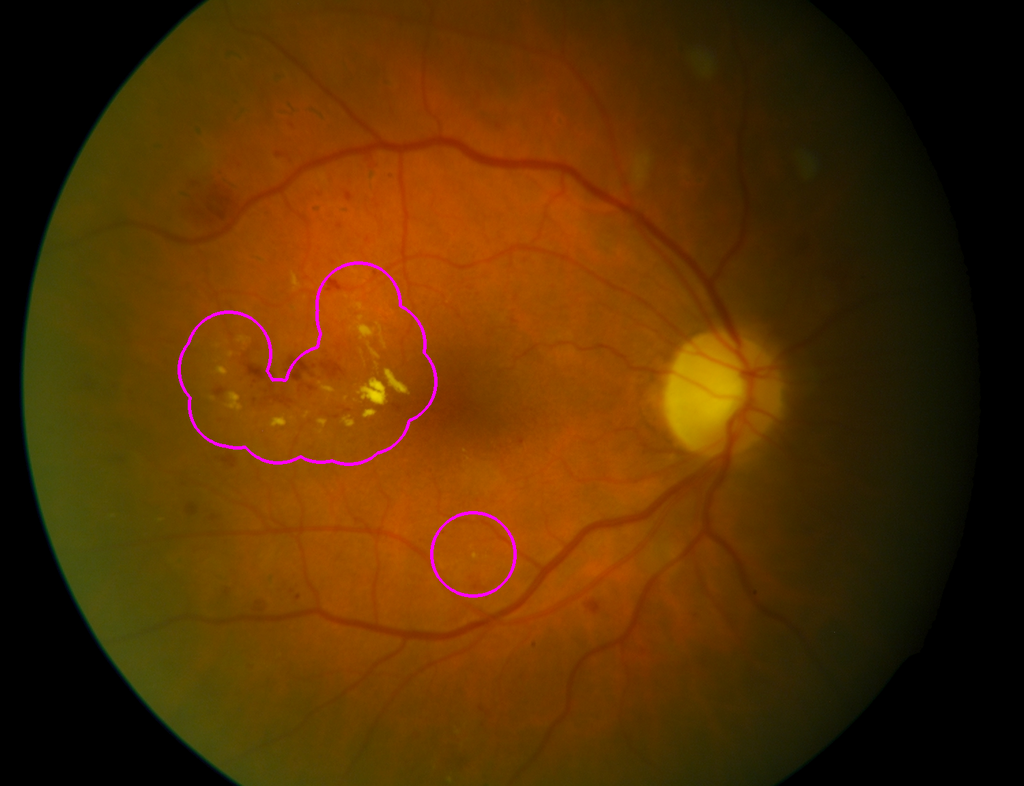
\includegraphics[width=.75\linewidth]{chap05_disease_result}
    \caption{Výsledek detekce.}
    \label{pic:chap05_disease_result}
  \end{center}
\end{figure}


\section{Výsledná struktura programu}
Navržený program pro automatickou detekci příznaků VPMD je implementován v~programovacím jazyce C++ s~využitím knihovny OpenCV. Mezi hlavní výhody této knihovny patří velké množství funkcí pro zpracování obrazu, které v~sobě zahrnuje, přenositelnost mezi různými operačními systémy a její volnou dostupnost pro akademické i komerční účely.

Výsledný program je rozdělen do několika souborů. Soubory \emph{detection.h} a \emph{detection.cpp} obsahují funkce implementující algoritmy, které byly navrženy výše. V~souborech \emph{tester.h} a \emph{tester.cpp} je implementována třída \emph{Tester} pro účely testování. Následující kapitola \ref{ch:testovani} obsahuje podrobnější popis funkce této třídy. Poslední hlavní soubor \emph{main.cpp} představuje vstupní bod programu, kde se zpracovávají vstupní argumenty, na jejichž základě se odvíjí další provádění programu.\par 

\bigskip\bigskip
\noindent\textbf{Přehled vstupních argumentů}\par\bigskip

\begin{tabularx}{\textwidth}{p{4cm}X}
  \textbf{-h, {-}{-}help}               & zobrazí nápovědu \\[5mm]
  \textbf{-i, {-}{-}image} \emph{path}   & vstupní snímek pro zpracování umístěný v~\emph{path} \\[5mm]
  \textbf{-d, {-}{-}detect}             & detekuje drúzy a exudáty \\[5mm]
  \textbf{{-}{-}mark}                   & vyznačí oblast optického disku a fovey \\[5mm]
  \textbf{{-}{-}mask}                   & zobrazí masku pozadí, optického disku a cév v~jediném snímku \\[5mm]
  \textbf{{-}{-}collect} \emph{database} & manuální lokalizace optického disku a fovey ve snímcích databáze \emph{database} pro vytvoření souboru \emph{groundtruth}\\[5mm]
  \textbf{{-}{-}test} \emph{groundtruth} & spuštění automatického testování detekce optického disku a fovey nad souborem \emph{groundtruth} \\[5mm]
  \textbf{{-}{-}compare} \emph{database} & postupné zobrazení všech snímků v~databázi \emph{database} a k~nim odpovídajících snímků s~detekovanými nálezy pro porovnání \\[5mm]
\end{tabularx}

\bigskip\bigskip
\noindent\textbf{Příklady spuštění}\par\bigskip

\begingroup
\setlength{\tabcolsep}{0pt}
\noindent\begin{tabularx}{\textwidth}{p{8.5cm}X}
  \emph{.{/}detector -i image001.png {-}{-}mask}               & zobrazí vstupní snímek spolu s~vytvořenou masku\\[5mm]
  \emph{.{/}detector -i image002.png {-}{-}mark {-}{-}detect}  & zobrazí vstupní snímek spolu se snímkem, na kterém je zaznačen optický disk, fovea a detekované nálezy\\[5mm]
  \emph{.{/}detector {-}{-}collect database{/}FIRE}            & vytvoří soubor \emph{groundtruth} v~adresáři databáze po manuální lokalizaci optického disku a fovey uživatelem\\[5mm]
  \emph{.{/}detector {-}{-}test database{/}FIRE{/}groundtruth} & spustí automatické testování ze souboru \emph{groundtruth} a do stejného adresáře vytvoří soubor \emph{test\_results} obsahující výsledky testování\\[5mm]
\end{tabularx}
\endgroup
  \chapter{Testování}
\label{ch:testovani}

\section{Zdrojové snímky}
Důležitým základem pro otestování algoritmu pro automatickou detekci příznaků onemocnění VPMD je mít dostatečně velké množství snímků sítnic. Tyto snímky by měly tvořit reprezentativní soubor zahrnující charakteristické příznaky tohoto onemocnění.

V~průběhu tvorby této práce byly využity databáze ADCIS \cite{db_adcis}, FIRE \cite{db_fire}, HRF \cite{db_hrf}, diaretdb0 \cite{db_diaret0} a diaretdb1 \cite{db_diaret1}. Databáze ADCIS je složena z~56 barevných digitálních snímků ve formátu JPG v~rozlišení 2544$\times$1696~pixelů a 1440$\times$960~pixelů. Z~těchto 56 snímků se na 37 vyskytují exudáty a zbylých 19 snímků zachycuje zdravé sítnice. Databáze FIRE obsahuje 42 snímků ve formátu JPG v~rozlišení 2912$\times$2912~pixelů. Tyto snímky taktéž zahrnují zdravé sítnice a sítnice s~těžkými exudáty. Databáze HRF je rozdělena na zdravé sítnice a sítnice obsahující příznaky diabetické retinopatie. Obě tyto skupiny obsahují 15 snímků s~rozlišením 3504$\times$2336~pixelů ve formátu JPG. Databáze diaretdb0 a diaretdb1 dohromady zahrnují 219 barevných digitálních snímků ve formátu PNG s~rozlišením 1500$\times$1152~pixelů obsahující nálezy jako neovaskularizaci, hemoragie a v~neposlední řadě také exudáty a drúzy. Další použitý soubor snímků byl pořízen na Fakultě informačních technologií v~Brně, která je vybavena vlastní fundus kamerou. Tento soubor obsahuje celkem 60 fotek sítnic, které byly pořízeny studenty. Tyto fotky neobsahují žádné příznaky VPMD. 

Dohromady je k~dispozici 407 snímků získaných pomocí fundus kamery. Souhrn informací o~těchto databázích je uveden v~tabulce \ref{tab:databases}.

Databáze ADCIS a FIRE obsahovaly velké množství obrázků zachycujících stejné sítnice, mezi kterými byly minimální rozdíly. Aby tyto podobné a opakující se obrázky nezkreslovaly výsledky testovaní, rozhodl jsem se pro jejich vyloučení.

\begin{table}[ht]
  \begin{center}	
    \begin{tabular}{|c|c|c|c|}
      \hline
      \textbf{Databáze} & \textbf{Rozlišení} & \textbf{Formát} & \textbf{Počet snímků} \\
      \hline
      ADCIS     & \makecell{2544$\times$1696\\ 1440$\times$960} & JPG &  56\\
      \hline
      FIRE      & 2912$\times$2912                            & JPG &  42\\
      \hline
      HRF       & 3504$\times$2336                            & JPG &  30\\
      \hline
      diaretdb0 & 1500$\times$1152                            & PNG & 130\\
      \hline
      diaretdb1 & 1500$\times$1152                            & PNG &  89\\
      \hline
      FIT       & 3888$\times$2592                            & JPG &  60\\
      \hline
      \multicolumn{3}{|r|}{$\sum$}                                   & 407\\
      \hline
    \end{tabular}
  \caption{Použité databáze.}
  \label{tab:databases}
  \end{center}
\end{table}


\section{Testování detekce optického disku a fovey}
Pro účely testování byla implementována samostatná třída \emph{Tester} poskytující metody pro sběr dat a jejich následné vyhodnocení. Tato třída využívá knihovny \emph{filesystem} pro rekurzivní procházení adresářové struktury obsahující snímky daných databází.

\subsection*{Sběr dat} 
V~prvním kroku je potřeba vytvořit referenční soubor dat, se kterým se budou porovnávat výsledky mého algoritmu. Člověk nemusí mít odborné znalosti očního lékaře pro lokalizaci optického disku a fovey na sítnici lidského oka a pouze stačí, pokud je informovaným laikem zasvěceným do této problematiky. Díky tomu jsem sběr dat pro testování detekce optického disku a fovey mohl provést sám bez nutnosti asistence oftalmologa. 

Testovací třída obsahuje metodu pro určení pozic těchto očních struktur uživatelem. Jako vstupní parametr této metody je předána cesta k~adresáři obsahující snímky určené k~testování. Všechny tyto snímky se postupně prochází a zobrazují se na obrazovce, kde uživatel prvním kliknutím levého tlačítka myši do obrázku určí střed optického disku a druhým kliknutím určí střed fovey. Získané polohy se ukládají do souboru \emph{groundtruth} umístěného v~adresáři dané databáze. Každý snímek má svůj záznam nacházející se na samostatném řádku, kde jsou středníkem odděleny jednotlivé informace. Nejprve se ukládá relativní cesta k~danému snímku vzhledem k~umístění tohoto souboru, následně jsou zaznamenány souřadnice optického disku a jako poslední jsou uloženy souřadnice fovey. Po druhém kliknutí myši a uložením daného záznamu se automaticky načte další obrázek. Takhle to probíhá do doby, než jsou zpracovány všechny snímky v~daném adresáři.

\subsection*{Vyhodnocení dat}
Další z~metod třídy \emph{Tester} realizuje samotné testování. Jako vstupní parametr je předána cesta ke \emph{groundtruth} souboru, který byl vytvořen v~předchozím kroku. Do jeho adresáře se vytvoří soubor \emph{test\_results} obsahující výsledky tohoto testování. 

Ze vstupního souboru se parsují jednotlivé záznamy, ze kterých se načtou konkrétní snímky. Každý tento snímek je předzpracován a následně je nad ním spuštěn algoritmus pro detekci optického disku. Získaná data se porovnávají s~daty obsaženými v~aktuálním záznamu. Porovnání je založeno na základě vzdálenosti ručně určeného středu se středem, který vypočítal algoritmus. 

Vzdálenost $|AB|$ dvou bodů $A[x_A, y_A]$ a $B[x_B, y_B]$ v~rovině je dána vzorcem:

\begin{equation}
  |AB| = \sqrt{(x_B - x_A)^2 + (y_B - y_A)^2}
\end{equation}

Pokud je vzdálenost mezi referenčním středem uvedeným v~záznamu a nalezeným středem optického disku menší než $2/3$ jeho poloměru, byl úspěšně detekován. Pokud je tato vzdálenost větší nebo rovna $2/3$ poloměru optického disku, detekce fovey se už netestuje, protože algoritmus pro její lokalizaci je závislý na umístění právě optického disku. Naopak v~případě jeho úspěšné lokalizace se detekce fovey spustí a následně se porovnává získaný střed s~referenčním středem, kde ke správné detekci došlo pouze v~případě, kdy jsou tyto středy od sebe vzdáleny maximálně do velikosti poloměru fovey.

Na konci souboru s~výsledky testování dané databáze je uvedena statistika. Z~ní lze vyčíst, na kolika snímcích byl úspěšně detekován optický disk z~jejich celkového počtu, na kolika fovea a jaká je celková úspěšnost jednotlivých algoritmů. Vzhledem k~tomu, že je detekce fovey závislá na lokalizaci optického disku, je zde uvedena i její úspěšnost vzhledem k~počtu správně nalezených optických disků.

\subsection*{Výsledky}
Výsledky detekce optického disku jsou shrnuty v~tabulce \ref{tab:results_od}. Většina nesprávných detekcí se nacházela na snímcích, které byly buď velmi špatně osvětleny, nebo obsahovaly optický disk, který splýval s~pozadím sítnice. 

Výsledky detekce fovey jsou shrnuty v~tabulce \ref{tab:results_fovea}, která obsahuje úspěšnost detekce vzhledem k~celkovému počtu snímků a také úspěšnost vzhledem k~celkovému počtu úspěšně detekovaných optických disků. Pokud se podaří správně lokalizovat optický disk, fovea je následně téměř vždy úspěšně nalezena. Po prozkoumání nesprávných detekcí z~výsledků vyplývá, že úspěšnost algoritmu je přímo úměrná kvalitě testovaných snímků. 

\begin{table}[ht]
  \begin{center}	
    \begin{tabular}{|c|c|c|}
      \hline
      \textbf{Databáze} & \textbf{Detekce} & \textbf{Úspěšnost}\\
      \hline
      ADCIS     & $53/56$   & 94,64 \% \\
      \hline
      FIRE      & $42/42$   & 100 \% \\
      \hline
      HRF       & $27/30$   & 90,00 \% \\
      \hline
      diaretdb0 & $119/130$ & 91,54 \% \\
      \hline
      diaretdb1 & $79/89$   & 88,76 \% \\
      \hline
      FIT       & $54/60$   & 90,00 \% \\
      \hline
      \hline
      \textbf{Celkem} & \textbf{374/407} & \textbf{91,89 \%} \\
      \hline
    \end{tabular}
  \caption{Výsledky testování detekce optického disku.}
  \label{tab:results_od}
  \end{center}
\end{table}

\begin{table}[ht]
  \begin{center}	
    \begin{tabular}{|c|c|c|c|c|}
      \hline
      \textbf{Databáze} & \textbf{Detekce} & \textbf{Úspěšnost} & \textbf{Detekce po úpravě} & \textbf{Výsledná úspěšnost}\\
      \hline
      ADCIS     & $51/56$   & 91,07 \% & $51/53$   & 96,23 \%\\
      \hline
      FIRE      & $41/42$   & 97,62 \% & $41/42$   & 97,62 \%\\
      \hline
      HRF       & $27/30$   & 90,00 \% & $27/27$   & 100 \%\\
      \hline
      diaretdb0 & $114/130$ & 87,69 \% & $114/119$ & 92,44 \%\\
      \hline
      diaretdb1 & $76/89$   & 85,39 \% & $76/79$   & 96,20 \%\\
      \hline
      FIT       & $54/60$   & 90,00 \% & $54/54$   & 100 \%\\
      \hline
      \hline
      \textbf{Celkem} & \textbf{363/407} & \textbf{89,19 \%} & \textbf{363/374} & \textbf{97.06 \%} \\
      \hline
    \end{tabular}
  \caption{Výsledky testování detekce fovey.}
  \label{tab:results_fovea}
  \end{center}
\end{table}


\section{Testování detekce drúz a exudátů}
Vyhodnocení úspěšnosti detekce nálezů jsem již nemohl provést sám, protože se poměrně těžce identifikují, proto je zapotřebí mít zkušenosti a odborné znalosti očního lékaře. Z~tohoto důvodu jsem si domluvil schůzku s~doktorem Tomášem Mňukem, který působí ve Fakultní nemocnici u~sv. Anny v~Brně a který mi velmi pomohl při klasifikaci těchto nálezů.

Testovací program postupně zobrazoval dva obrázky, kde první představoval výchozí nezměněný snímek a na druhém byly vyznačeny příznaky onemocnění detekované mým algoritmem. To lze vidět na obrázku \ref{pic:chap06_test_process}.

\begin{figure}[h]
  \begin{center}
    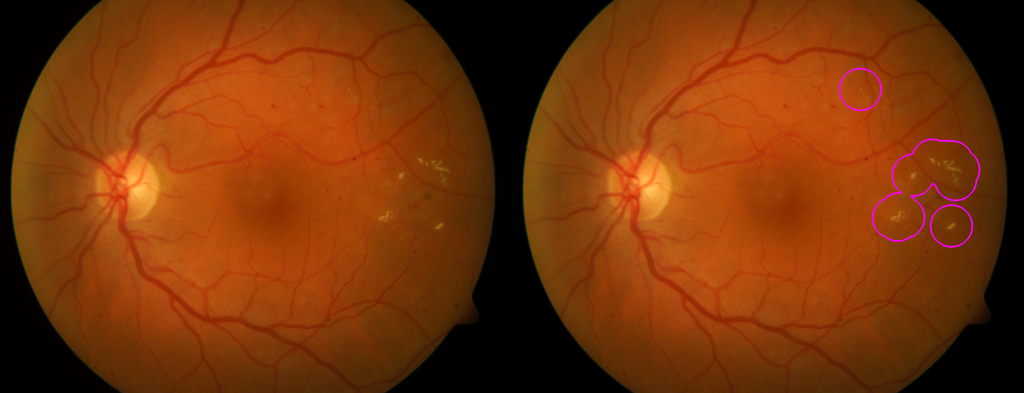
\includegraphics[width=\linewidth]{chap06_test_process}
    \caption{Testovací proces.}
    \label{pic:chap06_test_process}
  \end{center}
\end{figure}

Samotné vyhodnocování probíhalo manuálně, kde tyto snímky byly posouzeny doktorem. Ve vymezeném čase, který jsme spolu strávili, jsme však stihli otestovat pouze 50 snímků a to prvních 30 z~databáze diaretdb0 a prvních 20 z~databáze diaretdb1. Na snímcích se posuzovalo, zdali algoritmus správně detekoval drúzy a exudáty a zdali je detekoval všechny. Z~celkového počtu 50 snímků byly správně detekovány všechny drúzy či exudáty na 25, na 22 snímcích byla detekována většina, ale některé chyběly a na 3 snímcích byly kromě správných nálezů detekovány i oblasti, které nálezy nepředstavují. Hlavní příčinou nesprávné identifikace nálezů byla chyba při detekci krevního řečiště či optického disku. V~žádném z~případů se však nestalo, že by sítnice trpěla onemocněním VPMD nebo diabetické retinopatie a algoritmus by žádný z~příznaků nenalezl.

Já sám jsem již bez odborného dozoru provedl testování nad databázemi ADCIS a HRF, které jsou podle svého zdroje rozděleny na zdravé sítnice a sítnice s~nálezy, a souborem snímků sítnic pořízených na Fakultě informačních technologií v~Brně, u~kterého předpokládám, že obsahuje zdravé sítnice studentů. Dohromady bylo testováno 94 snímků, kde z~tohoto počtu byly na 21 snímcích nalezeny nějaké nálezy. Ty byly detekovány špatně a to hlavně z~důvodu, že se jednalo buď o~odlesky vzniklé špatným focením, nebo o~odlesky na sítnici, které se vyskytují u~mladých lidí. Podle pana doktora by však nemělo nastat, že by člověk trpěl VPMD a zároveň by měl na své sítnici tyto odlesky. Pokud by se tedy algoritmus použil pouze u~starších lidí, nemělo by k~těmto špatným detekcím docházet.

  \chapter{Závěr}
Věkem podmíněná makulární degenerace se řadí mezi nejčastější onemocnění sítnice lidského oka, proto bylo cílem této práce vymyslet a naimplementovat algoritmus pro automatickou detekci příznaků tohoto onemocnění, jehož včasná diagnóza je základem k~úspěšné léčbě. Tato práce poskytuje teoretický základ anatomie lidského oka a některých vybraných onemocnění sítnice. Z~technického hlediska se zaměřuje na různé metody zpracování digitálního obrazu a s~jejich využitím je navržen způsob detekce příznaků VPMD. V~závěru jsou zpracovány výsledky provedeného testování detekce optického disku, fovey a příznaků tohoto onemocnění.

Algoritmus začíná předzpracováním snímku následované získáním masky pozadí, která vymezí oblast sítnice pro další zpracování. Pomocí prahování se lokalizuje optický disk a následně fovea a pomocí adaptivního prahování se získá maska krevního řečiště. To vše je nezbytné pro odstranění nežádoucích oblastí ze zkoumaných snímků. Detekce příznaků je postavena na adaptivním prahování s~využitím malého okolí pixelů pro výpočet hodnot prahů jednotlivých pixelů. Tím se vymezí podezřelé oblasti. Ty jsou následně podrobeny analýze, která je klasifikuje na základě jejich barvy.

Testování bylo provedeno nad několika databázemi včetně souboru fotek pořízených na Fakultě informačních technologií v~Brně, což dohromady poskytlo 407 snímků sítnic. Toto testování bylo provedeno ve dvou formách, kde se v~první z~nich automaticky vyhodnocovala úspěšnost detekce optického disku a fovey na všech snímcích, která v~obou případech přesahovala hranici 90 \%. Ve druhé formě se manuálně za dozoru očního lékaře vyhodnocovala úspěšnost detekce příznaků u~50 snímků. Ve všech byla správně detekována přítomnost drúz či exudátů, ale ne vždy byly nalezeny všechny výskyty. U~tří sítnic byly dokonce nesprávně označeny prvky, které nepředstavují nálezy. Parametry programu v~průběhu testování jednotlivých databází nebyly nijak upravovány. Pro zajištění vyšší úspěšnosti by bylo nejlepší, kdyby se tyto parametry optimalizovaly pro konkrétní prostředí, ve kterém se budou dané snímky pořizovat.

Jedním z~možných praktických využití tohoto softwaru je jeho nasazení ve spojení s~fundus kamerou pro snímání sítnice. To pomůže lékařům k~rychlejšímu určení diagnózy a díky tomu k~včasnému zahájení léčby. Software by se dal využít i jako učební pomůcka pro oftalmology, kteří by si s~jeho pomocí procvičovali své znalosti. Díky vysoké úspěšnosti detekce základních struktur na sítnici by bylo možné tento software rozšířit o~detekci příznaků i jiných onemocnění, případně by mohl sloužit jako základ pro zcela novou aplikaci například z~oblasti biometrických systémů.
  
  % Použitá literatura
  % ----------------------------------------------
  \makeatletter
  \def\@openbib@code{\addcontentsline{toc}{chapter}{Literatura}}
  \makeatother
  \bibliographystyle{bib-styles/czechiso}

  \begin{flushleft}
  \bibliography{xaubre02_bibliography}
  \end{flushleft}

  % vynechání stránky v oboustranném režimu
  \iftwoside
    \cleardoublepage
  \fi


  % Přílohy
  % ---------------------------------------------
  \appendix
  \renewcommand{\appendixpagename}{Přílohy}
  \renewcommand{\appendixtocname}{Přílohy}
  \renewcommand{\appendixname}{Příloha}

  % vynechání stránky v oboustranném režimu
  \iftwoside
    \cleardoublepage
  \fi

  \chapter{Obsah přiloženého CD}
\label{cd_content}

Níže je zobrazena a popsána adresářová struktura nacházející se na přiloženém CD.

\begin{itemize}
  \item\textbf{databáze} - obsahuje jednotlivé databáze snímků sítnic

  \item\textbf{implementace}
    \begin{itemize}
      \item[$\circ$] \textbf{zdrojové soubory} - zdrojový kód programu
      \item[$\circ$] \textbf{dokumentace} - dokumentace zdrojového kódu (Doxygen)
      \item[$\circ$] \textbf{spustitelné soubory} - dva spustitelné soubory pro systémy Linux a Windows
    \end{itemize}

  \item\textbf{písemná zpráva}
    \begin{itemize}
      \item[$\circ$] \textbf{latex} - zdrojové soubory bakalářské práce pro vytvoření PDF souboru
      \item[$\circ$] \textbf{pdf} - bakalářská práce v PDF formátu
    \end{itemize}

  \item\textbf{testování}
    \begin{itemize}
      \item[$\circ$] \textbf{podklady} - kolekce \emph{groundtruth} souborů pro testování 
      \item[$\circ$] \textbf{výsledky} - výsledky automatického testování
    \end{itemize}  
\end{itemize}
  
\end{document}
